\section{Uncertainty Estimation for SAR Level-2 Products} \label{sec:level2}


This section expands the treatment of SAR-based Level-2 products.  

\subsection{Significant Wave Height}
\label{sec: SWH}

\subsubsection{Step 1: Definition of measurand, measurement model and retrieval model}
\label{sec: SWH model}

The uncertainty analysis of SAR-derived SWH discussed in this section is based on the linear relationship between the ``normalized'' azimuth wavelength cut-off ($\lambda_{C}^{20^{o}}$) and the
square root of the significant wave height ($H_{s}$), as described in Equation
\ref{eq: lc vs hs} \cite{GriecoIJRS2016}:

\begin{equation}
	\lambda_{C}^{20^{o}} = b_{0}+b_{1}\sqrt(H_{s})
	\label{eq: lc vs hs}
\end{equation}

\begin{equation}
   \lambda_{C}^{20^{o}} = \frac{R(\theta=20^{o})\sqrt{(F(\theta=20^{o},\phi_{0}=0^{o})}\lambda_{C})}{R(\theta)\sqrt{F(\theta,\phi_{o})}}
    \label{eq: lc20}
\end{equation}

As shown in Equation \ref{eq: lc20}$, \lambda^{20^{o}}_{C}$ depends on the slant range $R$, mean wave direction $\phi_{0}$ and the incidence angle $\theta$. $F$ is a trigonometric polynomial function, which is not reported here for the sake of brevity. The interested reader can refer to \cite{GriecoIJRS2016} for more details. 
$H_{s}$ can be obtained by simply inverting Equation \ref{eq: lc vs hs}, which leads to Equation \ref{eq: hs}.

\begin{equation}
	H_{s} = \left(\frac{\lambda^{20^{o}}_{C}-b_{0}}{b_{1}}\right)^{2}
	\label{eq: hs}
\end{equation}

The retrieval accuracy obtained with this algorithm is around 0.5 m, when compared against buoy measurements \cite{GriecoIJRS2016}. 
Note that $\lambda_{C}$, and so $\lambda_{C}^{20^{o}}$ is evaluated on 10x10 km$^{2}$ SAR sub-images.

\subsubsection{Step 2: Traceability Diagram}
\label{sec: UTD Hs}

Figure \ref{fig: SWH diag} shows the UTD, stressing both the measurement model of $\lambda_{C}^{20^{o}}$ and the retrieval model used. 

\begin{figure} [htbp]
    \centering
    \resizebox{\textwidth}{!}{
	\begin{tikzpicture}[
		% --- STILI ---
		node distance=0.7cm and 0.6cm,
		connection/.style={draw, thick},
		% Blocchi Principali
		root_block/.style={draw, rectangle, inner sep=10pt, font=\Large\bfseries, align=center},
		model_block/.style={draw, rectangle, inner sep=8pt, font=\large\bfseries, align=center},
		% Nodi Intermedi (Derivate)
		deriv_node/.style={draw, rectangle, rounded corners=5pt, inner sep=5pt, font=\normalsize, align=center},
		% Incertezze (Foglie)
		leaf_node/.style={draw, rectangle, inner sep=5pt, font=\small, align=center, text width=1.3cm},
		% Sorgenti (Effetti)
		effect_node/.style={draw, dashed, font=\footnotesize\itshape, align=center, text width=2.3cm, inner sep=3pt}
		]
		
		% --- ASSE CENTRALE ---
		% Modifica: lambda_C in rosso, b0 e b1 in blu (blue!70!black)
		\node [root_block] (CORE) {$H_s = \left( \frac{\textcolor{red}{\lambda_C^{20^\circ}} - \textcolor{blue!70!black}{b_0}}{\textcolor{blue!70!black}{b_1}} \right)^2 + 0$};
		
		\node [deriv_node, above=of CORE] (D_EQ9) {$\frac{\partial H_s}{\partial \lambda_C^{20^\circ}}$};
		
		\node [model_block, above=of D_EQ9] (EQ9) {$\lambda_C^{20^\circ} = \frac{\textcolor{purple}{R}(20^\circ)\sqrt{F(20^\circ, 0^\circ)}}{\textcolor{purple}{R}(\textcolor{cyan!80!black}{\theta})\sqrt{F(\textcolor{cyan!80!black}{\theta}, \textcolor{green!60!black}{\phi_0})}} \lambda_C(\textcolor{cyan!80!black}{\theta}, \textcolor{green!60!black}{\phi_0})$};
		
		\draw [connection, red] (CORE) -- (D_EQ9);
		\draw [connection, red] (D_EQ9) -- (EQ9);
		
		% --- INPUT SUPERIORI ---

		% 1. Distanza di Range (R)
		\node [deriv_node, above left=2.2cm and 3.2cm of EQ9] (D_R) {$\frac{\partial \lambda_C^{20^\circ}}{\partial R}$};
		\node [leaf_node, above=of D_R, draw=purple, text=purple] (U_R) {$u(R)$};
		\draw [connection, purple] (EQ9) -- (D_R);
		\draw [connection, purple] (D_R) -- (U_R);
		
		% 2. Angolo di Incidenza (Theta)
		\node [deriv_node, above left=2.2cm and 1.0cm of EQ9] (D_THETA) {$\frac{\partial \lambda_C^{20^\circ}}{\partial \theta}$};
		\node [leaf_node, above=of D_THETA, draw=cyan!80!black, text=cyan!80!black] (U_THETA) {$u(\theta)$};
		\draw [connection, cyan!80!black] (EQ9) -- (D_THETA);
		\draw [connection, cyan!80!black] (D_THETA) -- (U_THETA);

		% EFFETTI COMUNI per R e THETA
		\node [effect_node, above=0.5cm of $(U_R.north)!0.5!(U_THETA.north)$] (EFF_GEO) {Geolocation, \\ Orbital Fitting, \\ Antenna mis-pointing};
		\draw [connection, purple, dashed] (EFF_GEO) -- (U_R);
		\draw [connection, cyan!80!black, dashed] (EFF_GEO) -- (U_THETA);
		
		% 3. Misura Grezza (L_C)
		\node [deriv_node, above right=2.2cm and -1.cm of EQ9] (D_L_C) {$\frac{\partial \lambda_C^{20^\circ}}{\partial \lambda_C}$};
		\node [leaf_node, above=of D_L_C, draw=red, text=red] (U_L_C) {$u(\lambda_C)$};
        \node [effect_node, red, above=0.5cm of $(U_L_C.north)$] (EFF_U_L_C) {Bright Target Removal, \\ FFT, \\ CCS, \\ Range-averaging CCS, \\ IFFT, \\ Gaussian fit};
		\draw [connection, red, dashed] (EFF_U_L_C) -- (U_L_C);
		\draw [connection, red] (EQ9) -- (D_L_C);
		\draw [connection, red] (D_L_C) -- (U_L_C);
		
		% 4. Direzione del Vento (Phi_0)
		\node [deriv_node, above right=2.2cm and 1.8cm of EQ9] (D_PHI) {$\frac{\partial \lambda_C^{20^\circ}}{\partial \phi_0}$};
		\node [leaf_node, above=of D_PHI, draw=green!60!black, text=green!60!black] (U_PHI) {$u(\phi_0)$};
		\draw [connection, green!60!black] (EQ9) -- (D_PHI);
		\draw [connection, green!60!black] (D_PHI) -- (U_PHI);
		
		% EFFETTO per Phi_0
		\node [effect_node, green!60!black, above=0.5cm of U_PHI] (EFF_PHI) {NWP modelling};
		\draw [connection, green!60!black, dashed] (EFF_PHI) -- (U_PHI);
		
		% --- INPUT LATERALI (b0, b1 -> b) ---
		
		\node [deriv_node, right=0.8cm of CORE] (D_B) {$\frac{\partial H_s}{\partial \mathbf{b}}$};
		\node [leaf_node, right=0.5cm of D_B, draw=blue!70!black, text=blue!70!black] (U_B) {$u(\mathbf{b})$};
		\draw [connection, blue!70!black] (CORE) -- (D_B);
		\draw [connection, blue!70!black] (D_B) -- (U_B);
		
		% EFFETTO per b
		\node [effect_node, blue!70!black, above=0.3cm of U_B] (EFF_B) {Linear Fitting};
		\draw [connection, blue!70!black, dashed] (EFF_B) -- (U_B);
		
	\end{tikzpicture}
    }
    \caption{Uncertainty Tree Diagram with for $H_{s}$ retrieval.}
	\label{fig: SWH diag}
\end{figure}


\subsubsection{Step 3: Evaluation of sources of uncertainty}
\label{sec: Hs effects}

The error sources are described as follows:
\begin{itemize}
    \item $u(R)$: uncertainty in the slant range, which depends on the orbital fitting of the satellite platform;
    \item $u(\theta)$: uncertainty in the incidence angle, which also depends on the orbital fitting;
    \item $u(\phi_{0})$: uncertainty in the mean wave direction, which is input from Numerical Weather Prediction (\ac{NWP}) models;
	\item $u(b_{i})$: uncertainty of the offset and slope estimates of Equation \ref{eq: lc vs hs};
	\item $u(\lambda_{C})$: uncertainty of $\lambda_{C}$ estimate;
\end{itemize}

Note that $\lambda_{C}$ is estimated through several steps. Starting from
$\sigma_{0}$, all the steps for a SAR multi-look image are listed below:
\begin{itemize}
	\item Bright target removal. This step aims to remove bright spots that are supposed to be target echoes;
        \item \ac{FFT} of the \ac{SAR} sub-image of interest;
        \item Computation of \ac{CCS};
        \item Range-averaging of \ac{CCS};
        \item Computation of the \ac{CCF} through inverse \ac{FFT} of range-averaged \ac{CCS};
        \item Gaussian fit of \ac{CCF};
\end{itemize}

\noindent Each step is supposed to introduce additional errors, which finally affect $u(\lambda_{C})$. Figure \ref{fig: proc_diag_lambda20} shows the processing diagram for the steps mentioned above.

\begin{figure}[htbp]
	\centering
	\resizebox{\textwidth}{!}{
		\begin{tikzpicture}[
			node distance=1.0cm and 1.8cm,
			>=stealth,
			% --- STILI DA TABELLA 3.1 (DOCUMENTO NPL) ---
			dataset/.style={draw, trapezium, trapezium left angle=70, trapezium right angle=110, fill=white, font=\small\bfseries, align=center, minimum height=0.8cm},
			process/.style={draw, rectangle, fill=white, font=\small, align=center, minimum width=4.2cm, minimum height=0.8cm, inner sep=6pt},
			auxiliary/.style={draw, rounded rectangle, fill=gray!5, font=\small, align=center, minimum width=3.5cm},
			% --- FRECCE ---
			arrow/.style={->, thick, color=black!80}
			]
			
			% --- CATENA DI ELABORAZIONE LAMBDA_C (Sezione 5.3) ---
			\node [dataset] (IN_SAR) {SAR Multi-look Image \\ ($\sigma^0$)};
			
			\node [process, below=of IN_SAR] (STEP1) {1. Bright Target Removal};
			\node [process, below=of STEP1] (STEP2) {2. 2D FFT};
			\node [process, below=of STEP2] (STEP3) {3. Computation of CCS};
			\node [process, below=of STEP3] (STEP4) {4. Range-averaging of CCS};
			\node [process, below=of STEP4] (STEP5) {5. Inverse FFT (IFFT)};
			\node [process, below=of STEP5] (STEP6) {6. Gaussian fit of CCF};
			
			% Risultato intermedio
			\node [dataset, below=1.2cm of STEP6] (LAMBDA_C) {$\lambda_C$ Estimate};
			
			% --- NORMALIZZAZIONE (Equazione 5.2) ---
			
			% Dati ausiliari e di modello (Rettangolo arrotondato conforme a NPL)
			\node [auxiliary, right=of STEP4] (AUX_GEO) {Geometric and \\ Model Data ($R, \theta, \phi_0$)};
			
			\node [process, below=2.8cm of AUX_GEO, line width=0.8pt] (NORM) {Normalization \\ (Equation 5.2)};
			
			% Prodotto Finale (Parallelogramma)
			\node [dataset, below=1.2cm of NORM, fill=blue!2] (OUT_FINAL) {Normalized cut-off \\ $\lambda_{C}^{20^{\circ}}$};
			
			% --- COLLEGAMENTI ---
			\draw [arrow] (IN_SAR) -- (STEP1);
			\draw [arrow] (STEP1) -- (STEP2);
			\draw [arrow] (STEP2) -- (STEP3);
			\draw [arrow] (STEP3) -- (STEP4);
			\draw [arrow] (STEP4) -- (STEP5);
			\draw [arrow] (STEP5) -- (STEP6);
			\draw [arrow] (STEP6) -- (LAMBDA_C);
			
			% Ingressi per la normalizzazione
			\draw [arrow] (LAMBDA_C.east) -- ++(1,0) |- (NORM.west);
			\draw [arrow] (AUX_GEO) -- (NORM);
			\draw [arrow] (NORM) -- (OUT_FINAL);
			
			% Annotazioni laterali
			\node [anchor=west, font=\footnotesize\itshape, gray] at ($(STEP1.north east)+(0.2,0)$) {Azimuth wavelength cut-off ($\lambda_{C}$) estimation};
			\node [anchor=west, font=\footnotesize\itshape, gray] at ($(NORM.north east)+(0.2,0)$) {Normalization step};
			
		\end{tikzpicture}
	}
	\caption{Processing Diagram for the estimation of $\lambda_{C}^{20^{\circ}}$. The workflow combines SAR signal processing with auxiliary geometric and model-derived information ($R, \theta$ and $\phi_0$) to achieve the normalized output.}
	\label{fig: proc_diag_lambda20}
\end{figure}

Table \ref{tab: effects Hs} summarizes the uncertainty effects that finally affect the retrieval of $H_{s}$. \\
Note that $u(\lambda_{C})$ is evaluated on a single dataset \cite{GriecoIJRS2016}. Further studies are needed to assess this value with higher accuracy. \\
In addition, the uncertainty contribution from \(\lambda _{C}\) is assumed to be spatially independent (random) at the scale of the spectral estimation windows, as errors in the cut-off wavelength retrieval do not propagate across adjacent sub-images. \\
Finally, the spatial correlation scale of \(u(\lambda_C)\) is assumed to be zero at the macrocell level, implying instantaneous decorrelation between adjacent \(10 \times 10\text{ km}\) spectral estimation windows.\\
The uncertainties associated with the geometric parameters \(R\) and \(\theta \) are treated as spatially structured processes (structured) across the entire SAR image frame, as they originate from low-frequency orbital and attitude determination errors which remain highly correlated on a regional scale (Full scene). \\
The uncertainty of the auxiliary wind direction $\phi_{0}$ is driven by the spatial resolution and predictive skills of the underlying NWP model. Erroneous displacements of atmospheric features introduce highly correlated errors across regional scales. Therefore, its uncertainty is classified as structured with a spatial correlation scale of $\approx$100 km, while remaining independent (random) across different satellite passes. \\
The calibration coefficients \(b_{0}\) and \(b_{1}\) are static parameters derived from a global regression analysis. Their uncertainties do not vary across pixels, macrocells, or individual tracks, acting as a systematic bias for the entire product lifecycle. They are thus classified as structured across all spatial dimensions with a Global correlation scale, and temporally correlated until the next processor update (Full mission).

\begin{table}[h]
		\centering
		\scriptsize % Font ridotto per far entrare i 15cm
		\setlength{\tabcolsep}{2pt} % Riduce lo spazio tra le colonne
		\caption{Effects Table for $H_s$ retrieval}
		
		\begin{tabularx}{\textwidth}{l | X | X | X | X}
			\toprule
			\textbf{Name of effect} & Bright Target Removal, FFT, CCS, Range-averaging CCS, IFFT, Gaussian fit & Geolocation, Orbital fitting, Antenna mis-pointing & NWP modelling & Linear fitting \\
			\midrule
			\textbf{Effect Identifier} & 1.a.1.a & 1.a.2.a & 1.a.3.a & 1.b \\
			\midrule
			\textbf{Affected Term} & $\lambda_C$ & $R$, $\theta$ & $\phi_{0}$ & $b_0, b_1$ \\
			\midrule
			\textbf{Maturity} &  &  &  &  \\
			\quad -- Uncertainty & 1 & 3 & 3 & 1 \\
			\quad -- Correlation & 0 & 0 & - & - \\
			\quad -- Negligebility & No & Yes & No & Yes \\
			\midrule
			\textbf{Correlation type} &  &  &  &  \\
			\quad -- Along-track & random & structured & structured & structured \\
			\quad -- Cross-track & random & structured & structured & structured \\
			\quad -- Time & random & random & random & structured \\
			\midrule
			\textbf{Correlation scale} &  &  &  &  \\
			\quad -- Along-track & N/A & full scene & $\approx$100 km & Global \\
			\quad -- Cross-track & N/A & full scene & $\approx$100 km & Global \\
			\quad -- Time & N/A & N/A & N/A & Full mission \\
			\midrule
			\textbf{Uncertainty} & & & & \\
			\quad -- PDF shape & Gaussian & Gaussian & Gaussian & Bivariate \newline Gaussian \\
			\quad -- Units & m & m & deg & -- \\
			\quad -- Magnitude & $\sim$43m & Negligeable & $\sim$10$^\circ$ & $\sigma_{b_i}, \rho$ \\
			\midrule
			\textbf{Sensitivity coefficient} & $\frac{\partial H_s}{\partial \lambda_C^{20^{o}}} \frac{\partial \lambda_C^{20^{o}}}{\partial \lambda_C}$ & $\frac{\partial H_s}{\partial \lambda_C^{20^{o}}} \frac{\partial \lambda_C^{20^{o}}}{\partial R}$, $\frac{\partial H_s}{\partial \lambda_C^{20^{o}}} \frac{\partial \lambda_C^{20^{o}}}{\partial \theta}$ & $\frac{\partial H_s}{\partial \lambda_C^{20^{o}}} \frac{\partial \lambda_C^{20^{o}}}{\partial \phi_0}$ & $\frac{\partial H_s}{\partial b_i}$ \\
			\bottomrule
		\end{tabularx}
        \label{tab: effects Hs}
	\end{table}


\subsubsection{Step 4: Uncertainty Estimation}
\label{sec: Hs uncertainty}

In the following, the propagation of errors in the retrieval uncertainty is shown. We assume that the model errors in Equation \ref{eq: az cutoff} are Gaussian and independent of $H_{s}$. 
The total uncertainty $u_{H_s}$ is derived by combining the contributions of the measured parameter and the correlated fitting coefficients. The variance of $H_s$ is given by:
\begin{equation}
\begin{aligned}
    u_{H_s}^2 = & \left( \frac{\partial H_s}{\partial \lambda_C^{20^\circ}} \right)^2 u_{\lambda_C^{20^\circ}}^2 + \left( \frac{\partial H_s}{\partial b_0} \right)^2 u_{b_0}^2 + \left( \frac{\partial H_s}{\partial b_1} \right)^2 u_{b_1}^2 \\
    & + 2 \left( \frac{\partial H_s}{\partial b_0} \right) \left( \frac{\partial H_s}{\partial b_1} \right) \operatorname{cov}(b_0, b_1) + u_0^2 \\[15pt]
    u_{\lambda_C^{20^\circ}}^2 = & \left( \frac{\partial \lambda_C^{20^\circ}}{\partial \lambda_C} \right)^2 u_{\lambda_C}^2 + \left( \frac{\partial \lambda_C^{20^\circ}}{\partial R} \right)^2 u_R^2 + \left( \frac{\partial \lambda_C^{20^\circ}}{\partial \theta} \right)^2 u_\theta^2 + \left( \frac{\partial \lambda_C^{20^\circ}}{\partial \phi_0} \right)^2 u_{\phi_0}^2
\end{aligned}
\label{eq: errpro Hs}
\end{equation}

The sensitivity coefficients (partial derivatives) are:
\begin{equation}
\begin{aligned}
    \frac{\partial H_s}{\partial \lambda_C^{20^\circ}} &= \frac{2(\lambda_C^{20^\circ} - b_0)}{b_1^2} = \frac{2\sqrt{H_s}}{b_1} \\
    \frac{\partial H_s}{\partial b_0} &= -\frac{2\sqrt{H_s}}{b_1} \\
    \frac{\partial H_s}{\partial b_1} &= -\frac{2H_s}{b_1} \\
    \frac{\partial \lambda_C^{20^\circ}}{\partial \lambda_C} &= \frac{\lambda_C^{20^\circ}}{\lambda_C} \\ 
    \frac{\partial \lambda_C^{20^\circ}}{\partial R} &= -\frac{\lambda_C^{20^\circ}}{R(\theta)} \\ 
    \frac{\partial \lambda_C^{20^\circ}}{\partial \theta} &= -\frac{\lambda_C^{20^\circ}}{R(\theta)} \frac{\partial R}{\partial \theta} - \frac{\lambda_C^{20^\circ}}{2F} \frac{\partial F}{\partial \theta} \\
    \frac{\partial \lambda_C^{20^\circ}}{\partial \phi_0} &= -\frac{\lambda_C^{20^\circ}}{2F(\theta, \phi_0)} \frac{\partial F(\theta, \phi_0)}{\partial \phi_0}
\end{aligned}
\label{eq: parths}
\end{equation}

In the retrieval exercise shown in \cite{GriecoIJRS2016}, $u_{\lambda^{20^{o}}_{C}}\approx43$ m, and $b_0$ and $b_1$ equal to -93.66 m and 188.53 m$^{\frac{1}{2}}$, with standard deviations equal to 7.33 m and 4.25 m$^{\frac{1}{2}}$, respectively. Finally, the mutual correlation coefficient is equal to -0.98. Substituting these numbers in Equations \ref{eq: errpro Hs} and \ref{eq: parths}, we obtain retrieval uncertainties around 0.91 m for $H_{s}=4$ m. Note that most of this uncertainty is due to $u_{\lambda^{20^{o}}_{C}}$. \\
This is in line with the validation against ECMWF forecasts ($H_{s}^{for}$) shown in \cite{GriecoIJRS2016}. Figure \ref{fig: SWH pdf} shows the PDF of the $\hat{H}_{s}$ deviations from $H_{s}^{for}$ for the retrieval exercise shown in \cite{GriecoIJRS2016}. Some statistics are reported in the panel, namely bias, \ac{RMSD} and correlation coefficient ($\rho_{H_{s}}$). Note that the bias is very low and that the PDF is only slightly skewed; therefore, \ac{RMSD} is representative of the retrieval accuracy.

\begin{figure}
    \centering
    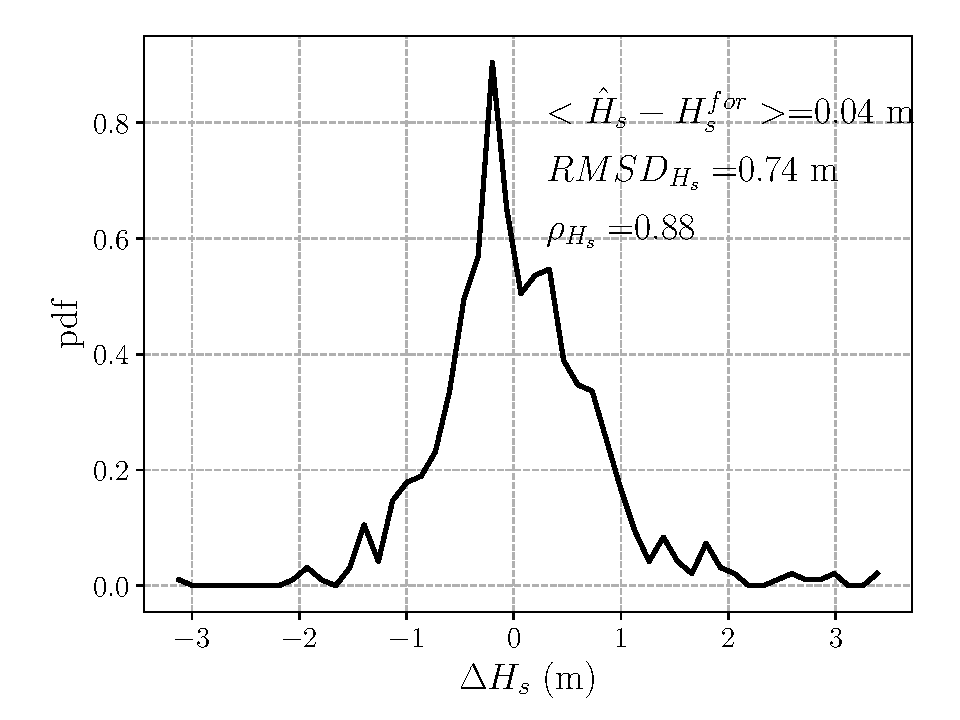
\includegraphics[width=0.8\linewidth]{figures/pdf_delta_Hs.pdf}
    \caption{Probability distribution function of the retrieved $H_{s}$ values.}
    \label{fig: SWH pdf}
\end{figure}

\subsection{Wind}
\label{sec: OSWV}

\subsubsection{Step 1: Definition of measurands, measurement models and retrieval model}
\label{sec: OSWV model}

The uncertainty analysis of SAR-derived \ac{OSWV} discussed in this section is presented for a Bayesian algorithm.  The a-posteriori conditional
\ac{PDF} of the retrieved \ac{OSWV} $\mathbf{\hat{v}}$ can
be modeled as reported in Equation \ref{eq: AP pdf}, which is a generalization
of the approach proposed in \cite{PortabellaJGRO2002}.

\begin{equation}
	\mathrm{pdf}_{\mathbf{v}|\sigma_{0},\varpi_{\rm dc},\lambda_{C},\mathbf{v_{B}}} \propto \mathrm{pdf}_{\mathbf{v}|\mathbf{v_{B}}} \mathrm{pdf}_{\sigma_{0}|\mathbf{v}} \mathrm{pdf}_{\lambda_{C}|U} \mathrm{pdf}_{\varpi_{\rm w}|\mathbf{v},\varpi_{\rm dc}}
	\label{eq: AP pdf}
\end{equation}

In Equation \ref{eq: Bayes}, $\sigma_{0}$ is the measured \ac{NRCS},
$\mathrm{pdf}_{\mathbf{v}|\mathbf{v_{B}}}$ is the conditional \ac{PDF} of
$\mathbf{v}$, known the a-priori (background) \ac{OSWV} $\mathbf{v_{B}}$,
$\mathrm{pdf}_{\sigma_{0}|\mathbf{v}}$ is the conditional \ac{PDF} of the
\ac{NRCS} prediction model, $\mathrm{pdf}_{\lambda_{C}|U}$ is the conditional
\ac{PDF} of the azimuth wavelength cut-off ($\lambda_{C}$) prediction model,
known the wind speed ($U$), and $\mathrm{pdf}_{\varpi_{\rm w}|\mathbf{v}}$ is
the conditional \ac{PDF} of the prediction model of the \ac{DCA} wind component
($\varpi_{\rm w}$), known \ac{DC} ($\varpi_{\rm dc}$). $\mathbf{v_{B}}$ is
provided by  \ac{NWP}, such as those from \ac{ECMWF}.

The optimal solution corresponds to the value $\mathbf{\hat{v}}$ that maximizes
the a-posteriori conditional \ac{PDF}.

Assuming that all \acp{PDF} are Gaussian, this is equivalent to minimize the
cost function reported in Equation \ref{eq: Bayes}

\begin{eqnarray}
	J = \frac{\sigma_{0}-\mathrm{GMF}_{\sigma_{0}}(\mathbf{v},\theta,\nu,pol)}{\Delta \sigma_{0}}+\frac{\mathbf{v}-\mathbf{v_{B}}}{\Delta \mathbf{v_{B}}}+ \nonumber \\
	\frac{\lambda_{C}-\mathrm{GMF}_{\lambda_{C}}(U,\theta,\nu,pol)}{\Delta \lambda_{C}}+\frac{\varpi_{\rm w}-\mathrm{GMF}_{\varpi_{\rm w}}(\mathbf{v},\theta,\nu,pol,\varpi_{\rm dc})}{\Delta \varpi_{\rm w}},
	\label{eq: Bayes}
\end{eqnarray}

\noindent where $\theta$ is the incidence angle, $\nu$ is the signal carrier
frequency, $pol$ is the polarization of the signal, and $\ac{GMF}$ stands
for Geophysical Model Function, which is the prediction model. As the name
suggests, a \ac{GMF} is an empirical forward model relating the geophysical
parameter domain to the observable domain. In this notation, the symbol
$\sigma_{0}$ states that \ac{NRCS} is averaged over a given area, typically of
1-2 km per side. This is required to mitigate wave modulation and reduce the
speckle \cite{MigliaccioJOE2007}. 

For a C-band \ac{SAR} such as Sentinel-1, CMOD7 \cite{StoffelenJSTARS2017} is used
as the \ac{NRCS} prediction model. The explicit formulation of CMOD7 is reported in
Equation \ref{eq: CMOD7} for the sake of completeness,

\begin{equation}
	\sigma_{0} = A_{0}(U,\theta) \left[1 + A_{1}(U, \theta) \cos(\phi)+A_{2}(U, \theta) \cos(2\phi) \right]^{1.6}
\label{eq: CMOD7}
\end{equation}

\noindent with $U$ the wind speed, $\phi$ the relative wind direction with
respect to the antenna looking angle, and $A_{i}, \ \forall i \in \left\{ 0,1,2
\right\}$, the fitting coefficients derived empirically. The dependency of the
coefficients $A_{i}$ on $\nu$ and $pol$ is implicit in this notation.


\subsubsection{Step 2: Traceability Diagram} \label{sec: OSWV UTD}

Figure \ref{fig: OSWV diag} shows the \ac{UTD}
for the \ac{OSWV} algorithm discussed in this section.

\begin{figure}
    \centering
	\resizebox{\textwidth}{!}{
	\begin{tikzpicture}[
		% --- DEFINIZIONE STILI GLOBALI (derivati dai tuoi blocchi) ---
		level distance=2cm,
		edge from parent/.style={draw, -, thick},
		root_main/.style={draw, rectangle, fill=gray!10, inner sep=10pt, font=\Large\bfseries, align=center},
		root_sub/.style={draw, rectangle, inner sep=8pt, font=\large\bfseries, align=center},
		node_black/.style={draw=black, rectangle, rounded corners, inner sep=5pt, font=\bfseries, text=black, align=center},
		node_model_red/.style={draw=red, rectangle, inner sep=5pt, font=\bfseries, text=black, align=center},
		node_model_blue/.style={draw=blue, rectangle, inner sep=5pt, font=\bfseries, text=black, align=center},
		node_model_green/.style={draw=green!50!black, rectangle, inner sep=5pt, font=\bfseries, text=black, align=center},
		leaf/.style={draw, rectangle, inner sep=4pt, font=\small, align=center, text width=1.2cm},
		effect/.style={draw, dashed, font=\tiny\itshape, align=center, text width=1.2cm, inner sep=2pt},
		connection/.style={draw, thick}
		]
		
		% --- NODO CENTRALE ---
		\node [root_main] (CORE) {$\mathbf{\hat{v}} = \arg\min_{\mathbf{v}} \sum_{i} J_i$};
		
		% --- BLOCCO 1: J_sigma0 (Posizionato in alto a sinistra) ---
		\node [root_sub, above left=6cm and 1cm of CORE] (J_SIGMA) {$J_{\sigma_{0}} = \left( \frac{\sigma_{0}^{M} - \sigma_{0}^{S}}{\Delta \sigma_{0}} \right)^2 + 0$}
		[sibling distance=2.5cm, level distance=1.4cm]
		child { node [node_black] (PAR_S0M) {$\frac{\partial J_{\sigma_{0}}}{\partial \sigma_{0}^{M}}$}
        edge from parent [draw=red]
			child { node [leaf, draw=red] (U_S0M) {$u(\sigma_0^{M})$} 
				node [effect, below=0.3cm of U_S0M] (EFF_S0M) {Radiometric cal., \\ SNR, \\ Speckle} } }
		child { node [node_black] {$\frac{\partial J_{\sigma_{0}}}{\partial \sigma_{0}^{S}}$}
			[sibling distance=2.cm, level distance=4.cm]
			child { node [node_model_red] {$\sigma_{0}^{S} = A_{0}\left[1+A_{1}cos(\phi)+A_{2}cos(2\phi)\right]^{p}$ + 0}
				[sibling distance=1.6cm, level distance=1.cm]
				child { node [node_black, font=\tiny] {$\frac{\partial \sigma_{0}^{S}}{\partial A_{i}}$} child { node [leaf, draw=red] (U_AI) {$u(A_i)$} 
						node [effect, below=0.3cm of U_AI] (EFF_UAI) {GMF fitting}
					} }
				child { node [node_black, font=\tiny] {$\frac{\partial \sigma_{0}^{S}}{\partial \theta}$} child { node [leaf, draw=red] (U_TH) {$u(\theta)$}   
						node [effect, below=0.3cm of U_TH] (EFF_TH) {Geolocation \\ Orbital Fitting \\ Antenna mis-pointing}
				} }
				child { node [node_black, font=\tiny] {$\frac{\partial \sigma_{0}^{S}}{\partial pol}$} child { node [leaf, draw=red] (U_POL) {$u(pol)$}  
						node [effect, below=0.3cm of U_POL] (EFF_POL) {Channel Cross-talk}
				} }
			}
			edge from parent [draw=red]
		}
		child { node [node_black] {$\frac{\partial J}{\partial \Delta \sigma_0}$}
			child { node [leaf, draw=red] {$u(\Delta \sigma_0)$} }
			edge from parent [draw=red]
		};
		\draw [connection, red, dashed] (EFF_POL) -- (U_POL);
		\draw [connection, red, dashed] (EFF_S0M) -- (U_S0M);
		\draw [connection, red, dashed] (EFF_UAI) -- (U_AI);
		\draw [connection, red, dashed] (EFF_TH) -- (U_TH);
		
		% --- BLOCCO 2: J_lambdaC (Posizionato in alto a destra) ---
		\node [root_sub, above right=6cm and -4cm of CORE] (J_LAMBDA) {$J_{\lambda_{C}} = \left( \frac{\lambda_{C}^{M} - \lambda_{C}^{S}}{\Delta \lambda_{C}} \right)^2 + 0$}
		[sibling distance=2.5cm, level distance=1.5cm]
		child { node [node_black] {$\frac{\partial J}{\partial \lambda_{C}^{M}}$}
			child { node [leaf, draw=blue] (U_LCM) {$u(\lambda_{C}^{M})$} 
				node [effect, below=0.3cm of U_LCM] (EFF_ULCM) {Bright Target Removal, \\ FFT, \\ CCS, \\ Range-averaging CCS, \\ IFFT, \\ Gaussian fit}
			}
			edge from parent [draw=blue]
		}
		child { node [node_black] {$\frac{\partial J}{\partial \lambda_{C}^{S}}$}
			child { node [node_model_blue] {$\lambda_{C}^{S} = \sum\limits_{i=0}^{1} a_{i}U_{i} + 0$}
				[sibling distance=1.6cm, level distance=1.5cm]
				child { node [node_black] {$\frac{\partial \lambda_{C}^{S}}{\partial \mathbf{a}}$} child { node [leaf, draw=blue] (U_a) {$u(\mathbf{a})$} 
						node [effect, right=0.3cm of U_a] (EFF_Ua) {linear fitting}
				} }
				edge from parent [draw=blue]
			}
			edge from parent [draw=blue]
		}
		child { node [node_black] {$\frac{\partial J}{\partial \Delta \lambda_{C}}$}
			child { node [leaf, draw=blue] {$u(\Delta \lambda_{C})$} }
			edge from parent [draw=blue]
		};
		\draw [connection, blue, dashed] (EFF_Ua) -- (U_a);
		\draw [connection, blue, dashed] (EFF_ULCM) -- (U_LCM);
		
		% --- BLOCCO 3: J_B (Posizionato in basso a sinistra) ---
		\node [root_sub, below left=2cm and 2cm of CORE] (J_BACK) {$J_{B} = \left( \frac{\mathbf{v} - \mathbf{v}_{B}}{\Delta \mathbf{v}_{B}} \right)^2 + 0$}
		[sibling distance=4cm, level distance=1.5cm]
		child { node [node_black] {$\frac{\partial J}{\partial \mathbf{v}_{B}}$}
			child { node [leaf, draw=orange!80!black] (U_VB) {$u(\mathbf{v}_{B})$} 
				node [effect, below=0.3cm of U_VB] (EFF_UVB) {NWP Modelling}
			}
			edge from parent [draw=orange!80!black]
		}
		child { node [node_black] {$\frac{\partial J}{\partial \Delta \mathbf{v}_{B}}$}
			child { node [leaf, draw=orange!80!black] {$u(\Delta \mathbf{v}_{B})$} }
			edge from parent [draw=orange!80!black]
		};
		\draw [connection, orange!80!black, dashed] (EFF_UVB) -- (U_VB);
		
		% --- BLOCCO 4: J_fw (Posizionato in basso a destra) ---
		\node [root_sub, below right=3cm and -6cm of CORE] (J_DOPP) {$J_{\varpi_{\rm w}} = \left( \frac{\varpi_{\rm w}^{M} - \varpi_{\rm w}^{S}}{\Delta \varpi_{\rm w}} \right)^2 + 0$}
		[sibling distance=5cm, level distance=1.5cm]
		child { node [node_black] {$\frac{\partial J_{\varpi_{\rm w}}}{\partial \varpi_{\rm w}^{M}}$}
			child { node [node_model_green, font=\tiny] {$\varpi_{\rm w}^{M} = \varpi_{\rm dc} - \varpi_{\rm elec} - \varpi_{\rm sca} - \varpi_{\rm att} - \varpi_{\rm ss} - \varpi_{\rm osc}+ 0$}
				[sibling distance=1.6cm, level distance=2.5cm]
                                child { node [node_black, font=\tiny] {$\frac{\partial \varpi_{\rm w}^M}{\partial \varpi_{\rm elec}}$} 
					[level distance=1.5cm]
					child { node [leaf, draw=green!50!black] (U_ELE) {$u(\varpi_{\rm elec})$} } }
                                        child { node [node_black, font=\tiny] {$\frac{\partial \varpi_{\rm w}^M}{\partial \varpi_{\rm att}}$} 
					[level distance=1.5cm]
					child { node [leaf, draw=green!50!black] (U_ATT) {$u(\varpi_{\rm att})$} 
						node [effect, below left =0.3cm and -0.65cm of U_ATT] (EFF_UATT) {Orbital Fitting, \\ Antenna mis-pointing}
					} }
                                        child { node [node_black, font=\tiny] {$\frac{\partial \varpi_{\rm w}^M}{\partial \varpi_{\rm ss}}$}
					[level distance=1.5cm] 
					child { node [leaf, draw=green!50!black] (U_SS) {$u(\varpi_{\rm ss})$} } }
                                        child { node [node_black, font=\tiny] {$\frac{\partial \varpi_{\rm w}^M}{\partial \varpi_{\rm osc}}$}
					[level distance=1.5cm] 
					child { node [leaf, draw=green!50!black] (U_OSC) {$u(\varpi_{\rm osc})$} 
						node [effect, below left =0.3cm and -0.65cm of U_OSC] (EFF_UOSC) {Sea state and \\ current modelling}
					} }
                                        child { node [node_black, font=\tiny] (PAR_FDCM) {$\frac{\partial \varpi_{\rm w}^M}{\partial \varpi_{\rm dc}}$} 
					[level distance=1.5cm] }
				edge from parent [draw=green!50!black]
			}
			edge from parent [draw=green!50!black]
		}
		child { node [node_black] {$\frac{\partial J_{\varpi_{\rm w}}}{\partial \varpi_{\rm w}^{S}}$}
			[sibling distance=5cm, level distance=2.5cm]
			child { node [node_model_green] {$\varpi_{\rm w}^{S} = GMF_{\varpi_{\rm w}}(\theta,\varpi_{\rm dc},pol,\nu) + 0$}
				[sibling distance=1.6cm, level distance=1.5cm]
				child { node [node_black] {$\frac{\partial \varpi_{\rm w}^{S}}{\partial \varpi_{\rm dc}}$} child { node [leaf, draw=green!50!black] (U_FDC) {$u(\varpi_{\rm dc})$}
						node [effect, below=0.3cm of U_FDC] (EFF_FDC) {Scene variability, \\ Scene size, \\ Speckle, \\ Scalloping, \\ SNR} 
				} }
				child { node [node_black] {$\frac{\partial \varpi_{\rm w}^{S}}{\partial \theta}$} child { node [leaf, draw=green!50!black] (U_TH2) {$u(\theta)$} 
						node [effect, below=0.3cm of U_TH2] (EFF_TH2) {Geolocation, \\ Orbital Fitting, \\ Antenna mis-pointing}
				} }
				edge from parent [draw=green!50!black]
			}
			edge from parent [draw=green!50!black]
		};
		\draw [connection, green!50!black, dashed] (EFF_FDC) -- (U_FDC);
		\draw [connection, green!50!black, dashed] (EFF_TH2) -- (U_TH2);
		\draw [connection, green!50!black, dashed] (EFF_UATT) -- (U_ATT);
		\draw [connection, green!50!black, dashed] (EFF_UATT) -- (U_ELE);
		\draw [connection, green!50!black, dashed] (EFF_UOSC) -- (U_OSC);
		\draw [connection, green!50!black, dashed] (EFF_UOSC) -- (U_SS);
		\draw [connection, green!50!black] (PAR_FDCM) -- (U_FDC);
		% --- CONNESSIONI AL CORE CENTRALE ---
		\draw [line width=2pt, red, -] (J_SIGMA.0) -| (CORE.163);
		\draw [line width=2pt, blue, -] (J_LAMBDA.0) -- ++(1,0) |- (CORE.0);
		\draw [line width=2pt, orange!80!black, -] (J_BACK.0) -| (CORE.240);
		\draw [line width=2pt, green!50!black, -] (J_DOPP.0) -| (CORE.340);
		
	\end{tikzpicture}
    }
\caption{Uncertainty Tree Diagram for the ocean surface wind vector retrieval algorithm presented.}
\label{fig: OSWV diag}
\end{figure}

\subsubsection{Step 3: Evaluation of sources of uncertainty}
\label{ref: OSWV effects}

In the first term of Equation \ref{eq: Bayes}, $\Delta \sigma_{0}$ is the
uncertainty of $\sigma_{0}$, which we may model as the sum of the
contributions from measurement uncertainty ($\Delta \sigma_{0}^{M}$) and
prediction model ($\Delta \sigma_{0}^{S}$).  The same contribution model
can be hypothesized for $\Delta \lambda_{C}=\Delta \lambda_{C}^{M}+\Delta
\lambda_{C}^{S}$ and $\Delta \varpi_{\rm w}=\Delta \varpi_{\rm w}^{M}+\Delta \varpi_{\rm w}^{S}$, which
represent the uncertainties of $\lambda_{C}$ and $\varpi_{\rm w}$, respectively.
Finally, $\Delta \mathbf{v_{B}}$ is the uncertainty of $\mathbf{v_{B}}$.

In the following treatment, the symbols $u$ and $\Delta$ have the same
meaning. We will use $\Delta$ for the terms explicitly stated in Equation \ref{eq: Bayes}. Therefore, the notation $u(\Delta \sigma_{0})$ stands for the uncertainty in the estimate of the uncertainty of $\sigma_{0}$.
Focusing on the first term of Equation \ref{eq: Bayes}, the following error
sources will contribute to the uncertainty of $J$:
\begin{itemize}
	\item $u(\sigma_{0})$: uncertainty of measured and simulated $\sigma_{0}$ values, namely $u(\sigma_{0}^{M})$ and $u(\sigma_{0}^{S})$, respectively. The first term depends on the instrument radiometric error, while the second depends on the accuracy of the prediction model (see next point);
	\item uncertainty of $\mathrm{CMOD7}$. The model is considered error-free. From a formal point of view, its deviation from reality is accounted for in the uncertainty of the coefficients $A_{i}$ ($u(A_{i})$);
	\item $u(\theta)$: uncertainty of the incidence angle. This can be due to errors in the model used to compute $\theta$, to antenna pointing errors, orbital fitting and geolocation. This error source is estimated to be very small;
	\item $u(\Delta \sigma_{0})$: uncertainty of $\Delta \sigma_{0}$ estimate. As said before, this quantity has two contributions, namely $u(\Delta \sigma_{0}^{M})$ and $u(\Delta \sigma_{0}^{S})$;
	\item $u(pol)$: uncertainty introduced by eventual signal leaking due to channel cross-talk. In the C-band, this error source is supposed to be small. This may not be the case of other spectral bands, such as L-band, due to signal interactions with the ionosphere; 
\end{itemize} 

\begin{table}[h]
	\centering
	\scriptsize % Font ridotto per far entrare i 15cm
	\setlength{\tabcolsep}{2pt} % Riduce lo spazio tra le colonne
	\caption{Effects Table for $J_{\sigma_{0}}$}
	
	\begin{tabularx}{\textwidth}{l | X | X | X | X}
		\toprule
		\textbf{Name of effect} & Radiometric Calibration, SNR, Speckle & GMF fitting & Geolocation, Orbital fitting, Antenna mis-pointing & Channel Cross-talk \\
		\midrule
		\textbf{Effect Identifier} & 1.a.1 & 1.b.1 & 1.b.2 & 1.b.3 \\
		\midrule
		\textbf{Affected Term} & $\sigma_{0}^{M}$ & $A_{i}$ & $\theta$ & $\sigma_{0}^{M}$ \\
		\midrule
		\textbf{Maturity} &  &  & & \\
		\quad -- Uncertainty & 3 & 3 & 3 & 2 \\
		\quad -- Correlation & 3 & N/A & 3 & TBD \\
		\quad -- Negligebility & No & No & No & No \\
		\midrule
		\textbf{Correlation type} &  &  & & \\
		\quad -- Along-track & random & structured & structured & structured \\
		\quad -- Cross-track & random & structured & structured & structured \\
		\quad -- Time & random & structured & random & random \\
		\midrule
		\textbf{Correlation scale} &  &  & & \\
		\quad -- Along-track & N/A & Global & Full scene & Full scene \\
		\quad -- Cross-track & N/A & Global & Full scene & Full scene \\
		\quad -- Time & N/A & Full mission & N/A & N/A \\
		\midrule
		\textbf{Uncertainty} & & & & \\
		\quad -- PDF shape & Negative Exponential & Gaussian & Gaussian & TBD \\
		\quad -- Units & dB & - & deg & dB \\
		\quad -- Magnitude & 0.2 dB & Negligeable & $\approx$0.01 deg & <-30 dB \\
		\midrule
		\textbf{Sensitivity Coefficient} & $\frac{\partial J_{\sigma_{0}}}{\partial \sigma_{0}^{M}}$ & $\frac{\partial J_{\sigma_{0}}}{\partial \sigma_{0}^{S}} \frac{\partial \sigma_{0}^{S}}{\partial A_{i}}$ & $\frac{\partial J_{\sigma_{0}}}{\partial \sigma_{0}^{S}} \frac{\partial \sigma_{0}^{S}}{\partial \theta}$ & $\frac{\partial J_{\sigma_{0}}}{\partial \sigma_{0}^{M}} \frac{\partial \sigma_{0}^{M}}{\partial pol}$ \\
		\bottomrule
	\end{tabularx}
	\label{tab: effects Js0}
\end{table}

In the second term of Equation \ref{eq: Bayes}, there are two sources of uncertainty:
\begin{itemize}
	\item $u(\mathbf{v_{B}})$: uncertainty of the background term;
	\item $u(\Delta \mathbf{v_{B}})$: uncertainty of the error source indicated in the previous point;
\end{itemize}

Table \ref{tab: effects JvB} reports the effects affecting $\mathbf{v_{B}}$. They are all summarized in ``\ac{NWP} modelling''. Making them more explicit is out of the scope of this document.

\begin{table}[h]
	\centering
	\scriptsize % Font ridotto per far entrare i 15cm
	\setlength{\tabcolsep}{2pt} % Riduce lo spazio tra le colonne
	\caption{Effects Table for $J_{\mathbf{v_{B}}}$}
	
	\begin{tabularx}{\textwidth}{l | X}
		\toprule
		\textbf{Name of effect} & NWP modelling \\
		\midrule
		\textbf{Effect Identifier} & 3.a \\
		\midrule
		\textbf{Affected Term} & $\mathbf{v_{B}}$ \\
		\midrule
		\textbf{Maturity} & \\
		\quad -- Uncertainty & 3 \\
		\quad -- Correlation & 3 \\
		\quad -- Negligebility & No \\
		\midrule
		\textbf{Correlation type} & \\
		\quad -- Along-track & structured \\
		\quad -- Cross-track & structured \\
		\quad -- Time & random \\
		\midrule
		\textbf{Correlation scale} & \\
		\quad -- Along-track & $\approx$100 km \\
		\quad -- Cross-track & $\approx$100 km \\
		\quad -- Time & N/A \\
		\midrule
		\textbf{Uncertainty} & - \\
		\quad -- PDF shape & Gaussian ($u,v$ components) \\
		\quad -- Units & ms$^{-1}$, deg \\
		\quad -- Magnitude & 1 ms$^{-1}$, $\approx$10$^{o}$ \\
		\midrule
		\textbf{Sensitivity Coefficient} & $\frac{\partial J_{\mathbf{v_{B}}}}{\partial \mathbf{v_{B}}}$ \\
		\bottomrule
	\end{tabularx}
	\label{tab: effects JvB}
\end{table}

In the third term, the additional error sources that have not been discussed before are listed below:
\begin{itemize}
	\item $u(\lambda_{C})$: uncertainty of the azimuth wavelength cut-off estimate. Here, $\lambda_{C}$ is considered ``normalized'', as written in Equation \ref{eq: lc20};
	\item $u(\Delta \lambda_{C})$: uncertainty of the previous error source;
	\item uncertainty of the prediction model ($\mathrm{GMF}_{\lambda_{C}}$). As shown in \cite{CorcioneTGRS2019,GriecoIJRS2016}, the dependency of $\lambda_{C}$ on $U$ is supposed to be linear in fully developed sea states, as written in Equation \ref{eq: az cutoff}:
	\begin{equation}
		\lambda_{C}=a+bU
		\label{eq: az cutoff}
	\end{equation}
	The deviation of the model from reality is accounted for in the uncertainty of the coefficients $a$ and $b$ ($u(a)$ and $u(b)$);
\end{itemize}

Table \ref{tab: effects JlC} summarizes the effects that affect $J_{\lambda_{C}}$, which is quite similar to table \ref{tab: effects Hs} introduced in Section \ref{sec: SWH} but for the name of the fitting coefficients.
\begin{table}[h]
		\centering
		\scriptsize % Font ridotto per far entrare i 15cm
		\setlength{\tabcolsep}{2pt} % Riduce lo spazio tra le colonne
		\caption{Effects Table for $J_{\lambda_{C}}$}
		
		\begin{tabularx}{\textwidth}{l | X | X | X | X}
			\toprule
			\textbf{Name of effect} & Bright Target Removal, FFT, CCS, Range-averaging CCS, IFFT, Gaussian fit & Geolocation, Orbital fitting, Antenna mis-pointing & NWP modelling & Linear fitting \\
			\midrule
			\textbf{Effect Identifier} & 2.a.1 & 2.a.2 & 2.a.3 & 2.b.1 \\
			\midrule
			\textbf{Affected Term} & $\lambda_C$ & $R$, $\theta$ & $\phi_{0}$ & $a, b$ \\
			\midrule
			\textbf{Maturity} &  &  &  &  \\
			\quad -- Uncertainty & 1 & 3 & 3 & 1 \\
			\quad -- Correlation & 0 & 0 & - & - \\
			\quad -- Negligebility & No & Yes & No & Yes \\
			\midrule
			\textbf{Correlation type} &  &  &  &  \\
			\quad -- Along-track & random & structured & structured & structured \\
			\quad -- Cross-track & random & structured & structured & structured \\
			\quad -- Time & random & random & random & structured \\
			\midrule
			\textbf{Correlation scale} &  &  &  &  \\
			\quad -- Along-track & N/A & full scene & $\approx$100 km & Global \\
			\quad -- Cross-track & N/A & full scene & $\approx$100 km & Global \\
			\quad -- Time & N/A & N/A & N/A & Full mission \\
			\midrule
			\textbf{Uncertainty} & & & & \\
			\quad -- PDF shape & Gaussian & Gaussian & Gaussian & Bivariate Gaussian \\
			\quad -- Units & m & m & deg & -- \\
			\quad -- Magnitude & $\sim$43m & Negligeable & $\sim$10$^\circ$ & $\sigma_{b_i}, \rho$ \\
			\midrule
			\textbf{Sensitivity coefficient} & $\frac{\partial J_{\lambda_{C}}}{\partial \lambda_C^{20^{o}}} \frac{\partial \lambda_C^{20^{o}}}{\partial \lambda_C}$ & $\frac{\partial J_{\lambda_{C}}}{\partial \lambda_C^{20^{o}}} \frac{\partial \lambda_C^{20^{o}}}{\partial R}$, $\frac{\partial J_{\lambda_{C}}}{\partial \lambda_C^{20^{o}}} \frac{\partial \lambda_C^{20}}{\partial \theta}$ & $\frac{\partial J_{\lambda_{C}}}{\partial \lambda_C^{20^{o}}} \frac{\partial \lambda_C^{20^{o}}}{\partial \phi_0}$ & $\frac{\partial J_{\lambda_{C}}}{\partial a}$, $\frac{\partial J_{\lambda_{C}}}{\partial b}$ \\
			\bottomrule
		\end{tabularx}
        \label{tab: effects JlC}
	\end{table}


In the last term, the additional error sources are:
\begin{itemize}
	\item $u(\varpi_{\rm dc})$: uncertainty of \ac{DC};
	\item $u(\varpi_{\rm elec})$: uncertainty due to antenna electronic mis-pointing;
	\item $u(\varpi_{\rm sca})$: uncertainty due to scalloping;
	\item $u(\varpi_{\rm att})$: uncertainty due to satellite attitude variations;
	\item $u(\varpi_{\rm osc})$: uncertainty of the estimate of the DCA ocean surface current component;
	\item $u(\varpi_{\rm ss})$: uncertainty of the estimate of the DCA sea state component;
\end{itemize}

\begin{table}[h]
		\centering
		\scriptsize % Font ridotto per far entrare i 15cm
		\setlength{\tabcolsep}{2pt} % Riduce lo spazio tra le colonne
		\caption{Effects Table for $J_{\varpi_{\rm w}}$}
		
		\begin{tabularx}{\textwidth}{l | X | X | X | X}
			\toprule
			\textbf{Name of effect} & Scene variability, Scene size, Speckle, Scalloping, SNR & Orbital fitting, Antenna mis-pointing & Sea State/Current modelling & GMF fitting \\
			\midrule
			\textbf{Effect Identifier} & 4.a & 4.b & 4.c & 4.b.1 \\
			\midrule
			\textbf{Affected Term} & $\varpi_{\rm dc}$ & $\varpi_{\rm p} \ (\varpi_{\rm att}$,$\varpi_{\rm elec})$ & $\varpi_{\rm ss}$,$\varpi_{\rm osc}$ & $\varpi_{\rm w}^{S}$ \\
			\midrule
			\textbf{Maturity} &  &  &  &  \\
			\quad -- Uncertainty & 3 & 3 & 3 & 3 \\
			\quad -- Correlation & 3 & 3 & 3 & 3 \\
			\quad -- Negligebility & No & No & No & No \\
			\midrule
			\textbf{Correlation type} &  &  &  &  \\
			\quad -- Along-track & random & structured & structured & structured \\
			\quad -- Cross-track & random & structured & structured & structured \\
			\quad -- Time & random & random & random & structured \\
			\midrule
			\textbf{Correlation scale} &  &  &  &  \\
			\quad -- Along-track & N/A & full scene & $\approx$100 km & Global \\
			\quad -- Cross-track & N/A & full scene & $\approx$100 km & Global \\
			\quad -- Time & N/A & N/A & N/A & full mission \\
			\midrule
			\textbf{Uncertainty} & & & & \\
			\quad -- PDF shape & Gaussian & Gaussian & Gaussian & Gaussian \\
			\quad -- Units & Hz & Hz & Hz & Hz \\
			\quad -- Magnitude & - & - & - & - \\
			\midrule
			\textbf{Sensitivity coefficient} & $\frac{\partial J_{\varpi_{\rm w}}}{\partial \varpi_{\rm w}^{M}} \frac{\partial \varpi_{\rm w}^{M}}{\partial \varpi_{\rm dc}}$ & $\frac{\partial J_{\varpi_{\rm w}}}{\partial \varpi_{\rm w}^{M}} \frac{\partial \varpi_{\rm w}^{M}}{\partial \varpi_{\rm elec,att}}$ & $\frac{\partial J_{\varpi_{\rm w}}}{\partial \varpi_{\rm w}^{M}} \frac{\partial \varpi_{\rm w}^{M}}{\partial \varpi_{\rm ss,osc}}$ & $\frac{\partial J_{\varpi_{\rm w}}}{\partial \varpi_{\rm w}^{S}}$ \\
			\bottomrule
		\end{tabularx}
        \label{tab: effects Jfw}
	\end{table}


\subsubsection{Step 4: Uncertainty Estimation}
\label{ref: OSWV uncertainty}

\begin{figure}[h]
	\centering
	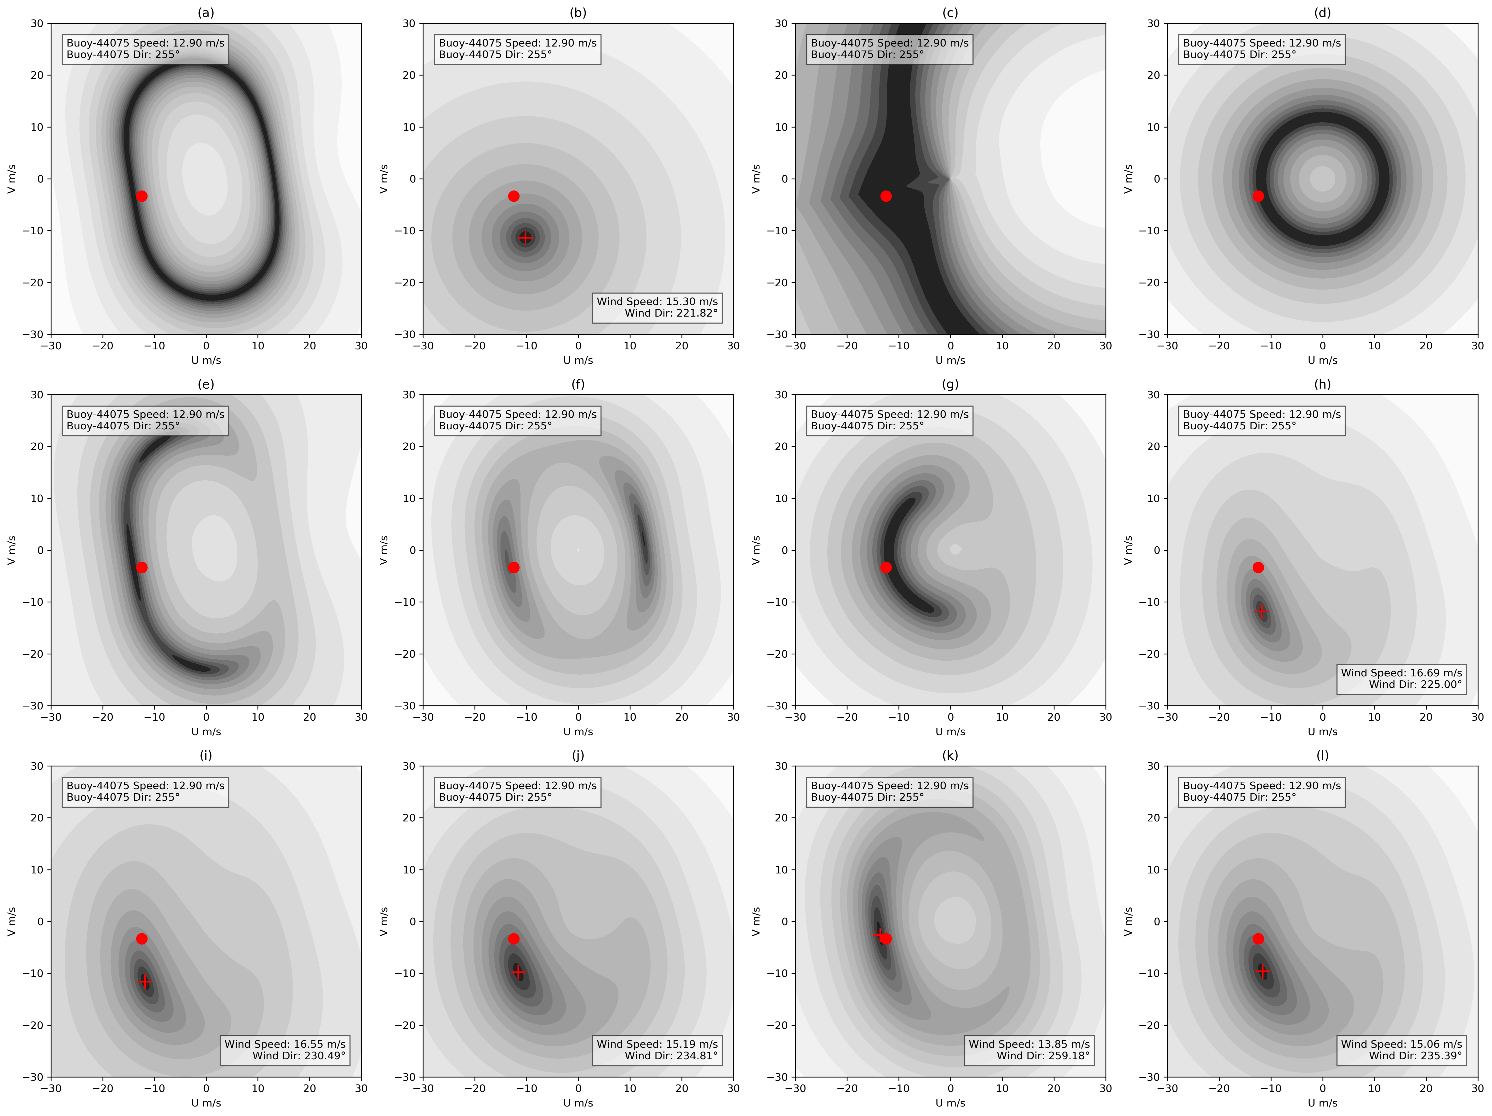
\includegraphics[width=.9\textwidth]{./figures/J}

        \caption{Cost function terms and their contributions. Darker shading
        indicates lower cost function values, representing a higher likelihood
        of the corresponding wind vector. Red circles denote the ``true'' wind
        vector from buoy observations, while red crosses indicate the wind
        vector obtained by minimizing the cost function. Subfigures (a)-(d)
        show individual contributions of \ac{NRCS}, background, Doppler, and azimuth
        wavelength cut-off terms. Subfigures (e)-(h) illustrate combined cost
        functions with, respectively, \ac{NRCS} and Doppler, \ac{NRCS} and azimuth
        wavelength cut-off, Doppler and azimuth wavelength cut-off terms, and
        \ac{NRCS} and background, highlighting ambiguities. Subfigures (i)-(l)
        present inversion results for various term combinations: (i)
        corresponds to the combination of \ac{NRCS}, Doppler and background, (j)
        that of \ac{NRCS}, azimuth wavelength cut-off and background, (k) that of
        \ac{NRCS}, Doppler and azimuth wavelength cut-off. Finally, (l) shows the
        combination of all terms in Equation \ref{eq: Bayes}.}

	\label{fig: J}
\end{figure}

The analytical propagation of input uncertainties through the Bayesian retrieval model (Equation \ref{eq: Bayes}) is highly non-linear and cannot be solved via a straightforward first-order Taylor expansion. 
In compliance with the GUM principles for non-linear minimization processes and the QA4EO general metrological framework, the quantitative uncertainty of the retrieved ocean surface wind vector \(\hat{\mathbf{v}} = [U, \phi]^T\) (wind speed and direction) is extracted numerically. Specifically, the combined standard uncertainty covariance matrix 
\(\mathbf{U}_{{\mathbf{\hat{v}}}}\) is derived from the inverse of the Hessian matrix (\(\mathbf{H}\)) of the total cost function \(J\), evaluated locally at the global minimum, which represents the optimal retrieval solution:
\begin{equation}
\mathbf{U}_{{\mathbf{\hat{v}}}}=\left[\begin{matrix}u^{2}(U)&\text{cov}(U,\phi )\\ \text{cov}(\phi ,U)&u^{2}(\phi )\end{matrix}\right]\approx \left(\frac{1}{2}\mathbf{H}(J)\right)^{-1}=\left(\frac{1}{2}\left[\begin{matrix}\frac{\partial ^{2}J}{\partial U^{2}}&\frac{\partial ^{2}J}{\partial U\partial \phi }\\ \frac{\partial ^{2}J}{\partial \phi \partial U}&\frac{\partial ^{2}J}{\partial \phi ^{2}}\end{matrix}\right]\right)_{\mathbf{v}={\mathbf{\hat{v}}}}^{-1}
\end{equation}
where the standard uncertainty for wind speed \(u(U)\) and relative wind direction \(u(\phi)\) are computed as the square roots of the diagonal elements of \(\mathbf{U}_{{\mathbf{\hat{v}}}}\). This numerical approach effectively projects the individual sensitivity coefficients and uncertainty magnitudes identified in Tables \ref{tab: effects Js0}, \ref{tab: effects JvB}, \ref{tab: effects JlC}, and \ref{tab: effects Jfw} onto the final Level-2 Thematic Data Product (TDP), mapping the localized constraints provided by the intersections of the cost function terms.
Figure \ref{fig: J} shows a retrieval case study using a Sentinel-1 \ac{SAR}
image acquired on January 17, 2022, at 22:43:11 UTC over the Atlantic Ocean
\cite{ZhuIGARSS2025}. As from the \ac{NDBC} buoy with ID
44075, wind speed and direction at 22:40 UTC measure 12.9 m$\cdot$s$^{-1}$ and
255$^{o}$, respectively, as also reported in the top-left corner of each
subplot. The collocated \ac{ERA5} wind speed and direction are
15.3 m$\cdot$s$^{-1}$ and 221.82$^{o}$, respectively. The buoy measurement and the
background winds are represented with a red circle and a cross, respectively,
in each plot.

Figure \ref{fig: J} shows the contribution of each term in Equation \ref{eq:
Bayes} to the cost function (top row) and the contribution of their
intersections two-to-two (central row) and three-to-three (first three plots of
the bottom row). Finally, the plot in the bottom right corner shows the total
cost function. Darker shading indicates lower cost function values,
representing a higher likelihood of the corresponding wind vector.

Figure \ref{fig: J}a shows an elliptical symmetry, with the major axes tilted
with respect to the north-south direction (v-axes). The inclination is due to
the satellite platform's flying direction, which is ascending in this specific
case. The along-track cross-track asymmetry is due to the bi-harmonic trend of
CMOD7, as depicted in Equation \ref{eq: CMOD7}. Given the measured
$\sigma_{0}$, the \ac{NRCS} term provides infinite solutions. This happens
because a conventional \ac{SAR} is a one-look instrument and has no azimuthal
look diversity, useful to reduce the number of ambiguities, such as in
scatterometers.

The background term has a sink shape, with the minimum in $\mathbf{v_{B}}$.
Note that the ``true'' and background winds are not very close. This may happen
in several situations, especially in rapidly changing weather patterns, such as
fronts and extreme events, but also due to the ``phase shift'' of \ac{NWP} models.
Finally, the low spatial resolution of \ac{NWP} models compared to \ac{SAR} plays a
non-negligible role \cite{VogelzangJGRO2011}. In these cases, the combination
of the \ac{NRCS} and background terms (Figure \ref{fig: J}h) can lead to
high-biased solutions, as thoroughly discussed in \cite{PortabellaJGRO2002}.

The Doppler term (Figure \ref{fig: J}c) appears quite complementary to the
\ac{NRCS} term, and helps to reduce ambiguities, as shown in Figure \ref{fig:
J}d. \\
Note that in this study, the Doppler components due to sea state and ocean surface current are neglected. This is equivalent to say that they are negligeable compared to the wind component. This assumption can be violated in areas with strong surface currents and/or swell. \\
When combined with the background term (Figure \ref{fig: J}i), the
a-posteriori \ac{PDF} has a well-defined peak \cite{MoucheTGRS2012}. However,
for the same reasons discussed before, this solution can be severely biased.

The azimuth wavelength cut-off term (Figure \ref{fig: J}d) shows a circular
symmetry. This is in agreement with the model introduced in Equation \ref{eq:
az cutoff}. Its combination with the \ac{NRCS} term can help to reduce
ambiguities, as shown in Figure \ref{fig: J}f, leading to a bi-modal
a-posteriori \ac{PDF}. However, this combination can be less fortunate, and the
peaks of the a-posteriori \ac{PDF} can be very spread, leading to a wide range
of ambiguities. In other words, the synergy between the \ac{NRCS} and azimuth
wavelength cut-off terms is not optimal. Instead, when these terms are combined
with the Doppler term, the solution converges towards the ``truth''. In this
specific case study, this solution is even better than what is obtained when
all terms are combined. Once more, this emphasizes the eventual biases of
\ac{NWP}. However, this is a fortunate case, which does not always happen. 

\subsection{Spatio-Temporal Collocation and Reference Uncertainties in Level-2 Ocean Validation}
\label{sec: spt errors}

In compliance with GUM principles regarding the evaluation of influence quantities within non-linear minimization and validation frameworks, the uncertainty budget of Level-2 Ocean products validated via Triple Collocation (TC) must account for the cross-platform representativeness error ($r^{2}$) and the sub-grid spatio-temporal mismatch uncertainty ($u_{\text{coll}}$). 

The operational selection of spatial ($\Delta x \le 25$ km) and temporal ($\Delta t \le 30$ min) boundaries for triplet integration introduces a localized geophysical noise component. This component stems from the fast-evolving nature of sub-mesoscale ocean boundary layer dynamics and wind-wave development, which cannot be assumed as stationary between the non-simultaneous satellite passes and physical in-situ sensor samplings.

The total collocated validation variance ($u^2$) is formally decomposed into three distinct metrological contributions:
\begin{equation}
u_{\text{val}}^2 = u_{\text{ret}}^2 + r^2 + u^{2}_{\Delta x, \Delta t}
\end{equation}

Where:
\begin{enumerate}
\item  $u_{ret}$ represents the intrinsic retrieval uncertainty.
\item  $r^{2}$ is the representativeness error, which captures the fundamental scale mismatch between a pointwise in-situ measurement and the footprint of spaceborne instruments, computed directly via spatial variance or spectral analysis.
\item  $u_{\Delta x, \Delta t}$ represents the specific uncertainty induced by the physical distance and time delay between the triplet observations.
\end{enumerate}

\subsection{Surface soil moisture}

This section sets up a framework for uncertainty analysis of Level-2 soil moisture
products derived from \ac{SAR} observations in an ESA/Copernicus context. The
framework is intended for a retrieved surface soil moisture quantity reported
per acquisition time and grid cell, with uncertainty information that remains
traceable to the calibrated radar observation, the inversion model, ancillary
data and the post-processing chain. The structure is consistent with established
\ac{SAR} soil-moisture retrieval literature, where calibration, incidence
angle, vegetation, roughness and representativeness are recurring contributors
to the uncertainty budget \cite{wagner07,zribi11,piles21,massart24}. In a
Copernicus context, this generic framework is also directly relevant to the
CLMS Surface Soil Moisture 1~km product and to downstream soil-water products
that ingest SAR-based near-surface moisture information \cite{clms_ssm1km,clms_swi}.

\paragraph{Step 1: Definition of measurand and measurement model}

The measurand is defined as the Level-2 surface soil moisture,
$\theta_{\rm sm}$, expressed in volumetric units (m$^3$/m$^3$), representative of
the sensed near-surface soil layer and of the spatial support of the product
cell. For a \ac{SAR}-based product, a generic measurement model may be written
as
\begin{equation}
  \theta_{\rm sm} = R(\sigma^0_{\rm cal}, \vartheta, x_{\rm aux}, p_{\rm ret}, c_{\rm pp}) + \Delta\theta_{\rm sm},
  \label{eq:sm_measurement_model}
\end{equation}
where $\sigma^0_{\rm cal}$ denotes the calibrated and geolocated radar
backscatter coefficient, $\vartheta$ is the local incidence angle and viewing
geometry, $x_{\rm aux}$ is the vector of ancillary inputs, $p_{\rm ret}$ is the
set of retrieval parameters and assumptions, $c_{\rm pp}$ denotes processing,
resampling and screening choices, and $\Delta\theta_{\rm sm}$ is the residual
uncertainty.

\noindent The ancillary vector $x_{\rm aux}$ may include land-cover class,
vegetation descriptors, surface roughness descriptors where available, digital
elevation information, soil texture and porosity, freeze/thaw state,
open-water fraction and masks required by the product specification. The
parameter set $p_{\rm ret}$ contains the coefficients, scattering-model choices
and empirical or semi-empirical assumptions used to invert the \ac{SAR}
observation into soil moisture. The term $c_{\rm pp}$ captures speckle
filtering, temporal compositing, spatial averaging, quality screening,
resampling and scaling where applicable.

\noindent For uncertainty propagation, it is useful to decompose the retrieval into
observation, ancillary and model terms as
\begin{equation}
  \theta_{\rm sm} = R\bigl(O(\sigma^0_{\rm raw}, g, n), A(z, m), p_{\rm ret}, c_{\rm pp}\bigr)
  + \Delta\theta_{\rm sm},
  \label{eq:sm_decomposition}
\end{equation}
where $O(\cdot)$ represents the observation operator including radiometric
calibration, terrain correction and geolocation, $A(\cdot)$ represents the
generation of ancillary inputs from external data $z$ and masks $m$, $g$
denotes geometric information and $n$ collects thermal noise, speckle and other
stochastic measurement errors.

\noindent Under a first-order GUM approximation, the combined variance of the
retrieved soil moisture may be written as
\begin{equation}
  u^2(\theta_{\rm sm}) \approx \sum_i \left(\frac{\partial \theta_{\rm sm}}{\partial x_i}\right)^2 u^2(x_i)
  + 2\sum_{i<j} \frac{\partial \theta_{\rm sm}}{\partial x_i}\frac{\partial \theta_{\rm sm}}{\partial x_j}\,\mathrm{cov}(x_i,x_j),
  \label{eq:sm_gum_propagation}
\end{equation}
where the input vector $x_i$ comprises, as appropriate, calibrated backscatter,
incidence angle, ancillary variables, retrieval parameters and post-processing
terms. This form is useful when the retrieval can be linearized locally around
the operating point and when correlation terms are available or can be
approximated.

\noindent For \mbox{L-band} \ac{SAR} systems such as NISAR and ROSE-L, the same
general framework applies, but additional attention is needed for increased
penetration into vegetation and the upper soil layer, stronger sensitivity to
forest and shrub canopies than at \mbox{C-band}, and potentially different
roughness and volume-scattering regimes. In practice, this means that the error
budget may require explicit terms for vegetation attenuation and structure,
subsurface scattering contributions, and transferability of retrieval
coefficients between \mbox{C-band} and \mbox{L-band} implementations. These are
well aligned with official mission descriptions emphasizing \mbox{L-band}'s
stronger vegetation penetration and land-surface sensitivity.

\paragraph{Step 2: Traceability diagram}

The corresponding uncertainty traceability can be organised as a tree rooted in
$\theta_{\rm sm}$. At the first level, the total uncertainty is separated into
contributions from the observation, the ancillary inputs, the retrieval model,
and the post-processing chain. A practical uncertainty tree for an ESA/Copernicus
Level-2 \ac{SAR} soil moisture product should contain at least the following
branches:
\begin{enumerate}
  \item \textbf{Observation branch:} radiometric calibration, thermal noise,
  speckle, geolocation, local incidence angle determination, terrain correction,
  shadow/layover handling and border-noise or artefact screening.
  \item \textbf{Ancillary-data branch:} land cover, vegetation descriptors,
  topographic information, soil texture, porosity, freeze/thaw and snow masks,
  and open-water fraction.
  \item \textbf{Retrieval-model branch:} scattering-model approximation,
  parameter fitting, correction for vegetation and roughness, transfer
  functions, possible saturation behaviour at very dry or very wet conditions,
  and model-form uncertainty.
  \item \textbf{Post-processing branch:} speckle filtering, temporal
  compositing, spatial resampling, gap filling, scaling to a reference data set,
  and quality filtering and flagging.
  \item \textbf{Representativeness branch:} mismatch between the sensor support,
  the product grid cell, the depth represented by the retrieval, and the target
  application variable used in validation or downstream data assimilation.
\end{enumerate}

\noindent The traceability diagram should support both pixel-level uncertainty and
correlation information. In particular, the analysis should explicitly describe
which effects are expected to be correlated in space, time and surface state.
For Copernicus products this is important because calibration, ancillary maps,
retrieval coefficients and topographic corrections can generate structured
uncertainties rather than purely random noise. Figure~\ref{fig:sm_uncertainty_trace}
shows a compact uncertainty tree diagram for the Level-2 \ac{SAR} soil moisture
product.

\begingroup
\hfuzz=2pt
\begin{figure*}[t]
  \centering
  \makebox[\textwidth][c]{\resizebox{0.92\textwidth}{!}{%
  \begin{tikzpicture}[node distance=8mm and 7mm, every node/.style={font=\footnotesize}]
    \node[draw,
          text width = 4.6cm,
          align = center,
          trapezium,
          trapezium left angle = 80,
          trapezium right angle = 100,
          trapezium stretches,
          minimum height=9mm] (sm) {$\theta_{\rm sm} = R(\sigma^0_{\rm cal}, \vartheta, x_{\rm aux}, p_{\rm ret}, c_{\rm pp}) + \Delta\theta_{\rm sm}$};

    \node[draw, above left = 10mm and 10mm of sm, text width = 3.5cm, align = center, minimum height=9mm] (obs)
      {$\sigma^0_{\rm cal} = O(\sigma^0_{\rm raw}, g, n) + \Delta\sigma^0$};
    \node[draw, left = 7mm of sm, text width = 9mm, align = center, minimum height=9mm] (dsmdobs)
      {$\frac{\partial\theta_{\rm sm}}{\partial\sigma^0_{\rm cal}}$};
    \node[draw, above = 7mm of obs, text width = 9mm, align = center, minimum height=9mm] (uobs) {$u(O)$};
    \node[left = 7mm of uobs, text width = 2.8cm, align = center] (obsleaf) {Calibration\\Thermal noise\\Speckle};

    \node[draw, above = 8mm of sm, text width = 9mm, align = center, minimum height=9mm] (dsmdgeom)
      {$\frac{\partial\theta_{\rm sm}}{\partial\vartheta}$};
    \node[draw, above = 8mm of dsmdgeom, text width = 3.1cm, align = center, minimum height=9mm] (geom)
      {$\vartheta = G(g, h_{\rm DEM}) + \Delta\vartheta$};
    \node[draw, above = 7mm of geom, text width = 9mm, align = center, minimum height=9mm] (ugeom) {$u(G)$};
    \node[right = 7mm of ugeom, text width = 2.7cm, align = center] (geomleaf) {Geolocation\\DEM uncertainty\\Topography};

    \node[draw, above right = 10mm and 10mm of sm, text width = 3.5cm, align = center, minimum height=9mm] (anc)
      {$x_{\rm aux} = A(z,m) + \Delta x_{\rm aux}$};
    \node[draw, right = 7mm of sm, text width = 9mm, align = center, minimum height=9mm] (dsmdanc)
      {$\frac{\partial\theta_{\rm sm}}{\partial x_{\rm aux}}$};
    \node[draw, above = 7mm of anc, text width = 9mm, align = center, minimum height=9mm] (uanc) {$u(A)$};
    \node[right = 7mm of uanc, text width = 2.8cm, align = center] (ancleaf) {Vegetation\\Land cover\\Freeze/thaw\\Soil texture};

    \node[draw, below left = 10mm and 10mm of sm, text width = 3.4cm, align = center, minimum height=9mm] (model)
      {$p_{\rm ret} = M(r_{\rm surf}, v_{\rm veg}) + \Delta p_{\rm ret}$};
    \node[draw, below = 7mm of dsmdobs, text width = 9mm, align = center, minimum height=9mm] (dsmdmodel)
      {$\frac{\partial\theta_{\rm sm}}{\partial p_{\rm ret}}$};
    \node[draw, below = 7mm of model, text width = 9mm, align = center, minimum height=9mm] (umodel) {$u(M)$};
    \node[left = 7mm of umodel, text width = 2.9cm, align = center] (modelleaf) {Roughness\\Vegetation correction\\Model-form uncertainty};

    \node[draw, below right = 10mm and 10mm of sm, text width = 3.3cm, align = center, minimum height=9mm] (pp)
      {$c_{\rm pp} = P(f_{\rm sp}, q, s) + \Delta c_{\rm pp}$};
    \node[draw, below = 7mm of dsmdanc, text width = 9mm, align = center, minimum height=9mm] (dsmdpp)
      {$\frac{\partial\theta_{\rm sm}}{\partial c_{\rm pp}}$};
    \node[draw, below = 7mm of pp, text width = 9mm, align = center, minimum height=9mm] (upp) {$u(P)$};
    \node[right = 7mm of upp, text width = 2.8cm, align = center] (ppleaf) {Filtering\\Resampling\\Quality screening\\Scaling};

    \draw[-latex] (obsleaf) edge (uobs) (uobs) edge (obs) (obs) edge (dsmdobs) (dsmdobs) edge (sm)
        (geomleaf) edge (ugeom) (ugeom) edge (geom) (geom) edge (dsmdgeom) (dsmdgeom) edge (sm)
        (ancleaf) edge (uanc) (uanc) edge (anc) (anc) edge (dsmdanc) (dsmdanc) edge (sm)
        (modelleaf) edge (umodel) (umodel) edge (model) (model) edge (dsmdmodel) (dsmdmodel) edge (sm)
        (ppleaf) edge (upp) (upp) edge (pp) (pp) edge (dsmdpp) (dsmdpp) edge (sm);
  \end{tikzpicture}%
  }}
  \caption{Uncertainty tree diagram for Level-2 \ac{SAR} soil moisture, $\theta_{\rm sm}$.}
  \label{fig:sm_uncertainty_trace}
\end{figure*}
\endgroup

\paragraph{Step 3: Evaluation of uncertainties}

Table~\ref{tab:sm_effects_table} provides a framework for documenting the main
uncertainty effects for a Level-2 \ac{SAR} soil moisture product. The table is intended to be completed during the product-specific error-budget analysis. The column headers denote effect categories rather than individual effects, and the rows labelled "Maturity" are placeholders to be populated during the product-specific assessment; they should not be interpreted as fixed maturity scores.

\begin{table}[ht]
  \scriptsize
  \centering

  \caption{Framework uncertainty effects table for Level-2 \ac{SAR} soil moisture,
  $\theta_{\rm sm}$.}

  \begin{tabular}{|l|c|c|c|c|c|c|}
    \hline
    \textbf{Effect category} & Observation & Geometry & Vegetation & Surface & Ancillary / & Total\\
    & noise/cal. & /topography & correction & model & post-proc. & product\\ \hline
    \textbf{Effect} &  &  &  &  & & \\
    \textbf{identifier} & 1 & 2 & 3 & 4 & 5 & 6 \\ \hline
    \textbf{Affected term} &  &  &  &  & & \\
    \textbf{term in} &  &  &  &  &  &\\
    \textbf{measurement} &  &  &  &  &  &\\
    \textbf{function} & $\sigma^0_{\rm cal}$ & $\vartheta$ & $x_{\rm veg}$ & $p_{\rm ret}$ & $x_{\rm aux}, c_{\rm pp}, R_{\rm sm}$ & $\theta_{\rm sm}$ \\ \hline
    \textbf{Maturity of} &  &  &  &  & & \\
    \textbf{analysis} & TBD & TBD & TBD & TBD & TBD & TBD \\ \hline
    Maturity of &  & &  &  & &  \\
    uncertainty &  & &  &  & &  \\
    estimate & TBD& TBD& TBD& TBD&TBD & TBD \\ \hline
    Maturity of &  & &  &  & &  \\
    correlation scale &  & &  &  & &  \\
    estimate & TBD& TBD& TBD& TBD& TBD& TBD \\ \hline
    For low maturity, &  & &  &  & &  \\
    is effect negligible? & No & No & No & No & No & No\\ \hline
    \textbf{Correlation type} &  & &  &  &  &\\
    \textbf{and form} &  & &  &  &   &\\ \hline
    Range/cross-track & TBD & TBD & TBD & TBD & TBD & TBD \\ \hline
    Azimuth/along-track & TBD & TBD & TBD & TBD & TBD & TBD \\ \hline
    Over time & TBD & TBD & TBD & TBD & TBD & TBD \\ \hline
    Between land-cover classes & TBD & TBD & TBD & TBD & TBD & TBD \\ \hline
    \textbf{Correlation scale} &  & & &  &  &  \\ \hline
    Space & TBD & TBD & TBD & TBD & TBD & TBD\\ \hline
    Time & TBD & TBD & TBD & TBD & TBD & TBD\\ \hline
    Conditions & TBD & TBD & TBD & TBD & TBD & TBD \\ \hline
    \textbf{Uncertainty} &  & &  &  &&  \\ \hline
    PDF shape & TBD & TBD & TBD & TBD & TBD & TBD \\ \hline
    Units & input units & radians/deg & input units & input units & input units & m$^3$/m$^3$ \\ \hline
    Magnitude & TBD & TBD & TBD & TBD & TBD & TBD \\ \hline
    \textbf{Sensitivity} & & & &  &  &  \\
    \textbf{coefficient} & $\frac{\partial\theta_{\rm sm}}{\partial \sigma^0_{\rm cal}}$ & $\frac{\partial\theta_{\rm sm}}{\partial \vartheta}$ & $\frac{\partial\theta_{\rm sm}}{\partial x_{\rm veg}}$ & $\frac{\partial\theta_{\rm sm}}{\partial p_{\rm ret}}$ & branch-wise / combined & 1 \\ \hline
  \end{tabular}

  \label{tab:sm_effects_table}
\end{table}

\noindent In a product-specific implementation, the evaluation should distinguish
between Type-A components estimated statistically from repeat observations or
matchups, and Type-B components derived from calibration knowledge, model
assumptions, ancillary-data specifications and expert judgement. The total
uncertainty reported with the Level-2 product should state clearly whether it is
an estimate of retrieval uncertainty, representativeness uncertainty, or a
combined quantity.

\noindent In particular, a surface-soil-moisture product should not
automatically receive low maturity scores in every branch: observation
calibration and parts of the retrieval model may be comparatively mature,
whereas correlation-scale estimates, representativeness terms and some
ancillary or post-processing effects may still have substantially lower
maturity.

\noindent For ESA/Copernicus delivery, the final analysis should also document:
\begin{enumerate}
  \item the product definition, including sensing depth, spatial support and
  masking rules;
  \item the list of uncertainty components that are included and excluded;
  \item the propagation method, whether analytical, ensemble-based or Monte
  Carlo;
  \item the treatment of spatial and temporal correlations; and
  \item the validation strategy against in situ networks and reference products.
\end{enumerate}

\subsection{Surface Wet Snow}

This section applies the same general methodology to a Level-2 Surface Wet Snow
product derived from \ac{SAR}. In contrast to soil moisture, the measurand is
not a continuous geophysical variable but a categorical class assigned to each
pixel or grid cell. The uncertainty analysis must therefore address both the
quality of the underlying radar evidence and the probability of classification
errors between the classes \texttt{WET}, \texttt{NO-WET} and \texttt{MASK}.

\paragraph{Step 1: Definition of measurand and measurement model}

The measurand is defined as the surface wet-snow state, $S_{\rm ws}$,
classified into the mutually exclusive categories
\begin{equation}
  S_{\rm ws} \in \{\mathrm{WET},\, \mathrm{NO\mbox{-}WET},\, \mathrm{MASK}\}.
  \label{eq:wetsnow_classes}
\end{equation}
A generic classification model can be written as
\begin{equation}
  S_{\rm ws} = C(\sigma^0_{\rm cal}, \Delta\sigma^0, \vartheta, x_{\rm aux}, t_{\rm ref}, q) + \Delta S_{\rm ws},
  \label{eq:wetsnow_measurement_model}
\end{equation}
where $\sigma^0_{\rm cal}$ is the calibrated and geolocated \ac{SAR}
backscatter, $\Delta\sigma^0$ denotes the change metric relative to a dry-snow
or reference state where such a method is used, $\vartheta$ is the local
incidence angle and geometry, $x_{\rm aux}$ collects masks and ancillary data,
$t_{\rm ref}$ denotes reference-period information, $q$ is the decision logic
or threshold set, and $\Delta S_{\rm ws}$ represents residual classification
uncertainty. This formulation is consistent with the classical multitemporal
SAR wet-snow change-detection approach and with later Sentinel-1-based
extensions that combine backscatter change with auxiliary information and
terrain constraints \cite{nagler00,tsai19}.

\noindent In this case, the uncertainty analysis should not rely only on standard
error propagation for a continuous variable. Instead, it should explicitly
address probabilities of false wet detection, missed wet snow, and erroneous
masking. The natural output quantities are therefore class probabilities,
confusion-matrix elements, or confidence scores associated with each class.

\noindent A useful intermediate quantity is a continuous decision variable,
$D_{\rm ws}$, for example based on a backscatter change metric and ancillary
screening:
\begin{equation}
  D_{\rm ws} = F(\sigma^0_{\rm cal}, \Delta\sigma^0, \vartheta, x_{\rm aux}, t_{\rm ref}),
  \label{eq:wetsnow_decision_variable}
\end{equation}
with the final class assignment obtained from thresholding and masking logic,
\begin{equation}
  S_{\rm ws} = C(D_{\rm ws}, q, m),
  \label{eq:wetsnow_classification_rule}
\end{equation}
where $q$ denotes thresholds or class boundaries and $m$ denotes the relevant
mask set. For this product, uncertainty is therefore better characterized
through class-transition probabilities such as $P(\mathrm{WET}\!\mid\!\mathrm{NO\mbox{-}WET})$,
$P(\mathrm{NO\mbox{-}WET}\!\mid\!\mathrm{WET})$, and $P(\mathrm{MASK}\!\mid\!\cdot)$ than through a
single variance alone.


Figure~\ref{fig:wetsnow_sigmoid_concept} illustrates a more concrete
interpretation of these transition probabilities for the common wet-snow
change-detection case in which the decision variable is based on the
backscatter difference relative to a dry-snow reference. The horizontal axis is
therefore written as $\Delta\sigma^0$ in dB. A nominal wet/no-wet threshold is
shown at $-3$~dB, which is a commonly used order-of-magnitude threshold in SAR
wet-snow detection, while the smooth crossing of the curves illustrates how
uncertainty can still be represented probabilistically around the threshold.

\begin{figure}[ht]
  \centering
  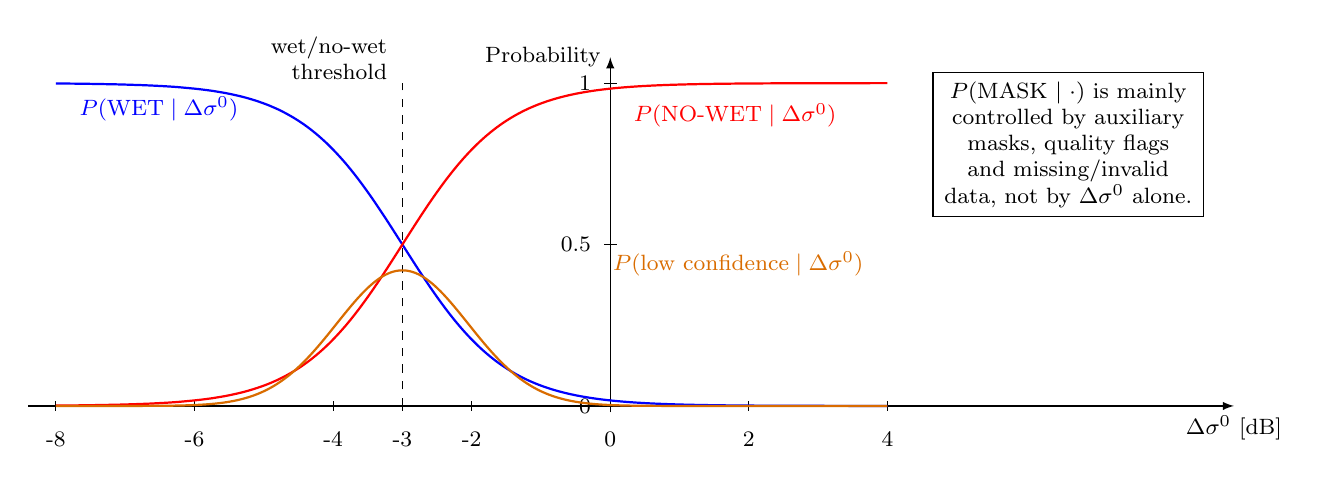
\begin{tikzpicture}[x=0.88cm,y=4.1cm,font=\footnotesize]
    \draw[-latex] (-8.4,0) -- (9.0,0) node[below] {$\Delta\sigma^0$ [dB]};
    \draw[-latex] (0,-0.02) -- (0,1.08) node[left] {Probability};

    \foreach \y/\label in {0/0,0.5/0.5,1/1}
      \draw (-0.09,\y) -- (0.09,\y) node[left=2mm] {\label};

    \foreach \x/\label in {-8/-8,-6/-6,-4/-4,-3/-3,-2/-2,0/0,2/2,4/4}
      \draw (\x,0.015) -- (\x,-0.015) node[below=1.5mm] {\label};

    \draw[dashed] (-3,0) -- (-3,1.0);
    \node[above left, align=right] at (-3.08,0.98) {wet/no-wet\\threshold};

    \draw[thick,blue,samples=150,smooth,domain=-8:4] plot(\x,{1/(1+exp(1.35*(\x+3)))});
    \draw[thick,red,samples=150,smooth,domain=-8:4] plot(\x,{1 - 1/(1+exp(1.35*(\x+3)))});
    \draw[thick,orange!85!black,samples=150,smooth,domain=-8:4] plot(\x,{0.42*exp(-((\x+3)*(\x+3))/1.8)});

    \node[blue,anchor=west] at (-7.8,0.92) {$P(\mathrm{WET}\mid \Delta\sigma^0)$};
    \node[red,anchor=west] at (0.2,0.9) {$P(\mathrm{NO\mbox{-}WET}\mid \Delta\sigma^0)$};
    \node[orange!85!black,anchor=west] at (-0.1,0.44) {$P(\mathrm{low\ confidence}\mid \Delta\sigma^0)$};

    \node[draw,align=center,anchor=west,text width=3.2cm] at (4.65,0.81)
      {$P(\mathrm{MASK}\mid\cdot)$ is mainly controlled by auxiliary masks,\ quality flags and missing/invalid data, not by $\Delta\sigma^0$ alone.};
  \end{tikzpicture}
  \caption[Conceptual wet-snow transition probabilities]{Conceptual wet-snow transition probabilities versus backscatter difference relative to a dry-snow reference. The blue and red curves indicate soft class probabilities for \texttt{WET} and \texttt{NO-WET}, crossing near the nominal threshold $\Delta\sigma^0=-3$~dB. The orange curve marks a low-confidence region around the threshold. The mask probability is shown separately as an auxiliary gating process rather than as a direct sigmoid of $\Delta\sigma^0$.}
  \label{fig:wetsnow_sigmoid_concept}
\end{figure}

\noindent In the Copernicus HR-S\&I ATBD, the operational WDS and SWS processing is
specified through hierarchical decision rules and QC layers propagated from the
intermediate SAR wet-snow detection rather than through an explicit sigmoid
probability model. In particular, the ATBD describes QCISWS as the quality
layer of the intermediate SAR wet-snow map, and the final QCSSC and QCWSM
layers inherit or mask this QC information through rule-based product
generation. The probability curves in Figure~\ref{fig:wetsnow_sigmoid_concept}
should therefore be read as a conceptual uncertainty representation of the
threshold behaviour, while $P(\mathrm{MASK}\mid\cdot)$ is better interpreted as a
separate auxiliary-data-driven gating probability.

\paragraph{Categorical products and latent continuous counterparts}

For categorical Level-2 products, uncertainty should generally not be expressed
only by an overall accuracy or a single confusion matrix. A more informative
representation is to report class-membership probabilities, entropy or margin-
based confidence measures, together with class-wise omission/commission rates
and, where relevant, their spatial variation \cite{ibrahim05,loosvelt12,comber12,roodposhti19}.

\noindent Conceptually, many categorical products can be interpreted as a discretized
view of an underlying continuous or mixed latent variable. In statistical terms,
this corresponds to threshold or latent-variable formulations in which observed
classes arise from a continuous propensity, or to mixture formulations in which
categorical and continuous latent structure coexist \cite{liu17,lubke08}.

\noindent For wet snow, the most natural continuous counterpart is not the class label
itself but the underlying thermodynamic and dielectric state of the snowpack,
of which liquid water content (LWC) is one important descriptor. Field studies
show that LWC is spatially and temporally heterogeneous even within apparently
similar wetness conditions \cite{techel11,bonnell21}. Radar studies likewise show
that wet-snow detectability depends on volumetric liquid water content together
with geometry and surface conditions \cite{magagi03}.

\noindent It follows that a Surface Wet Snow class should be understood as an indirect
decision on a latent state rather than as a one-to-one observation of LWC. In
practice, the correspondence between a wet-snow class and LWC is many-to-one:
different LWC values, vertical water distributions or melt-refreeze conditions
may map to the same class, while similar LWC values may fall on different sides
of the class boundary because of forest cover, roughness, incidence angle or
reference-state mismatch. For uncertainty analysis, this means that class
probability and latent-state uncertainty should ideally be distinguished. A
product may therefore report (i) the probability of the class \texttt{WET}, and,
where a retrieval model exists, (ii) an auxiliary estimate or interval for a
continuous wetness descriptor such as LWC or a decision variable monotonically
related to LWC.


\paragraph{Step 2: Traceability diagram}

The uncertainty tree for surface wet snow should separate the following main
branches:
\begin{enumerate}
  \item \textbf{Observation branch:} radiometric calibration, thermal noise,
  speckle, geolocation, terrain correction, incidence-angle normalization and
  screening of border or artefact effects.
  \item \textbf{Reference-state branch:} uncertainty in the dry-snow reference,
  temporal representativeness of the reference image or climatology, and
  seasonal drift in the backscatter baseline.
  \item \textbf{Decision-logic branch:} threshold selection, model coefficients,
  class-boundary sensitivity and hysteresis effects near the wet/no-wet
  threshold.
  \item \textbf{Ancillary-mask branch:} land mask, forest mask, glacier mask,
  layover/shadow mask, water mask, snow mask and quality flags.
  \item \textbf{Representativeness branch:} mismatch between pixel-scale radar
  response and the target class definition, including sub-pixel mixtures,
  vegetation cover, topographic heterogeneity and diurnal melt-refreeze
  variability.
\end{enumerate}

\noindent For a categorical product, the traceability analysis should also identify
which effects primarily cause confusion between \texttt{WET} and
\texttt{NO-WET}, and which effects tend to move samples into \texttt{MASK}.
This is especially important because topography, forest cover and rapid temporal
changes in snow conditions can produce structured classification errors rather
than independent pixel noise. Figure~\ref{fig:wetsnow_uncertainty_trace} shows a
compact uncertainty tree diagram for the Level-2 Surface Wet Snow product. For
Copernicus implementation, the most directly relevant operational references
are the CLMS SAR Wet Snow (SWS) and Wet/Dry Snow (WDS) products, which provide
the product-level context for the uncertainty components listed here
\cite{clms_sws,clms_wds}.

\begin{figure*}[t]
  \centering
  \begin{tikzpicture}[scale=0.88, transform shape, node distance=8mm and 7mm, every node/.style={font=\footnotesize}]
    \node[draw,
          text width = 4.8cm,
          align = center,
          trapezium,
          trapezium left angle = 80,
          trapezium right angle = 100,
          trapezium stretches,
          minimum height=9mm] (snow) {$S_{\rm ws} = C(\sigma^0_{\rm cal}, \Delta\sigma^0, \vartheta, x_{\rm aux}, t_{\rm ref}, q) + \Delta S_{\rm ws}$};

    \node[draw, above left = 10mm and 10mm of snow, text width = 3.3cm, align = center, minimum height=9mm] (obs)
      {$\sigma^0_{\rm cal} = O(\sigma^0_{\rm raw}, g, n) + \Delta\sigma^0_{\rm cal}$};
    \node[draw, left = 7mm of snow, text width = 9mm, align = center, minimum height=9mm] (dcdobs)
      {$\frac{\partial C}{\partial\sigma^0_{\rm cal}}$};
    \node[draw, above = 7mm of obs, text width = 9mm, align = center, minimum height=9mm] (uobs) {$u(O)$};
    \node[left = 7mm of uobs, text width = 2.8cm, align = center] (obsleaf) {Calibration\\Thermal noise\\Speckle\\Terrain correction};

    \node[draw, above = 8mm of snow, text width = 9mm, align = center, minimum height=9mm] (dcdref)
      {$\frac{\partial C}{\partial\Delta\sigma^0}$};
    \node[draw, above = 8mm of dcdref, text width = 3.3cm, align = center, minimum height=9mm] (ref)
      {$\Delta\sigma^0 = B(\sigma^0_{\rm cal}, t_{\rm ref}) + \Delta\Delta\sigma^0$};
    \node[draw, above = 7mm of ref, text width = 9mm, align = center, minimum height=9mm] (uref) {$u(B)$};
    \node[right = 7mm of uref, text width = 2.8cm, align = center] (refleaf) {Dry-snow reference\\Seasonal drift\\Temporal mismatch};

    \node[draw, above right = 10mm and 10mm of snow, text width = 4.2cm, align = center, minimum height=9mm] (mask)
      {$x_{\rm aux} = A(m_{\rm snow}, m_{\rm lay}, m_{\rm water}) + \Delta x_{\rm aux}$};
    \node[draw, right = 7mm of snow, text width = 9mm, align = center, minimum height=9mm] (dcdmask)
      {$\frac{\partial C}{\partial x_{\rm aux}}$};
    \node[draw, above = 7mm of mask, text width = 9mm, align = center, minimum height=9mm] (umask) {$u(A)$};
    \node[right = 7mm of umask, text width = 2.8cm, align = center] (maskleaf) {Forest mask\\Water mask\\Layover/shadow\\Snow mask};

    \node[draw, below left = 10mm and 10mm of snow, text width = 3.2cm, align = center, minimum height=9mm] (decision)
      {$q = Q(\tau, h, r) + \Delta q$};
    \node[draw, below = 7mm of dcdobs, text width = 9mm, align = center, minimum height=9mm] (dcdq)
      {$\frac{\partial C}{\partial q}$};
    \node[draw, below = 7mm of decision, text width = 9mm, align = center, minimum height=9mm] (uq) {$u(Q)$};
    \node[left = 7mm of uq, text width = 2.7cm, align = center] (qleaf) {Thresholds\\Hysteresis\\Class-boundary sensitivity};

    \node[draw, below right = 10mm and 10mm of snow, text width = 3.8cm, align = center, minimum height=9mm] (repr)
      {$R_{\rm ws} = H(f_{\rm sub}, v_{\rm forest}, t_{\rm diel}) + \Delta R_{\rm ws}$};
    \node[draw, below = 7mm of dcdmask, text width = 9mm, align = center, minimum height=9mm] (dcdrepr)
      {$\frac{\partial C}{\partial R_{\rm ws}}$};
    \node[draw, below = 7mm of repr, text width = 9mm, align = center, minimum height=9mm] (urepr) {$u(H)$};
    \node[right = 7mm of urepr, text width = 2.9cm, align = center] (reprleaf) {Sub-pixel mixture\\Forest cover\\Topography\\Melt-refreeze cycle};

    \draw[-latex] (obsleaf) edge (uobs) (uobs) edge (obs) (obs) edge (dcdobs) (dcdobs) edge (snow)
        (refleaf) edge (uref) (uref) edge (ref) (ref) edge (dcdref) (dcdref) edge (snow)
        (maskleaf) edge (umask) (umask) edge (mask) (mask) edge (dcdmask) (dcdmask) edge (snow)
        (qleaf) edge (uq) (uq) edge (decision) (decision) edge (dcdq) (dcdq) edge (snow)
        (reprleaf) edge (urepr) (urepr) edge (repr) (repr) edge (dcdrepr) (dcdrepr) edge (snow);
  \end{tikzpicture}
  \caption{Uncertainty tree diagram for Level-2 Surface Wet Snow classification, $S_{\rm ws}$.}
  \label{fig:wetsnow_uncertainty_trace}
\end{figure*}

\paragraph{Step 3: Evaluation of uncertainties}

Table~\ref{tab:wetsnow_effects_table} gives a corresponding framework for the
uncertainty analysis of a Level-2 Surface Wet Snow product. As for Table~\ref{tab:sm_effects_table}, the columns denote effect categories, while the maturity rows are placeholders to be filled with product-specific assessments rather than default zero scores.

\begin{table}[ht]
  \scriptsize
  \centering

  \caption{Framework uncertainty effects table for Level-2 Surface Wet Snow
  classification, $S_{\rm ws}$.}

  \begin{tabular}{|l|c|c|c|c|c|c|}
    \hline
    \textbf{Effect category} & Observation & Reference & Decision & Ancillary & Representa- & Total\\
    & /calibration & state & logic & masks & tiveness & classification\\ \hline
    \textbf{Effect} &  &  &  &  & & \\
    \textbf{identifier} & 1 & 2 & 3 & 4 & 5 & 6 \\ \hline
    \textbf{Affected term} &  &  &  &  & & \\
    \textbf{term in} &  &  &  &  &  &\\
    \textbf{measurement} &  &  &  &  &  &\\
    \textbf{function} & $\sigma^0_{\rm cal}$ & $t_{\rm ref}, \Delta\sigma^0$ & $q$ & $x_{\rm aux}$ & $R_{\rm ws}$ & $S_{\rm ws}$ \\ \hline
    \textbf{Maturity of} &  &  &  &  & & \\
    \textbf{analysis} & TBD & TBD & TBD & TBD & TBD & TBD \\ \hline
    Maturity of &  & &  &  & &  \\
    uncertainty &  & &  &  & &  \\
    estimate & TBD& TBD& TBD& TBD&TBD & TBD \\ \hline
    Maturity of &  & &  &  & &  \\
    correlation scale &  & &  &  & &  \\
    estimate & TBD& TBD& TBD& TBD& TBD& TBD \\ \hline
    For low maturity, &  & &  &  & &  \\
    is effect negligible? &  No& No&  No&  No&  No& No\\ \hline
    \textbf{Correlation type} &  & &  &  &  &\\
    \textbf{and form} &  & &  &  &   &\\ \hline
    Space & TBD & TBD & TBD & TBD & TBD & TBD \\ \hline
    Over time & TBD & TBD & TBD & TBD & TBD & TBD \\ \hline
    Between snow regimes & TBD & TBD & TBD & TBD & TBD & TBD \\ \hline
    Between classes & TBD & TBD & TBD & TBD & TBD & TBD \\ \hline
    \textbf{Classification quality} &  & & &  &  &  \\ \hline
    False-wet rate & TBD & TBD & TBD & TBD & TBD & TBD\\ \hline
    Missed-wet rate & TBD & TBD & TBD & TBD & TBD & TBD\\ \hline
    False-mask rate & TBD & TBD & TBD & TBD & TBD & TBD \\ \hline
    \textbf{Uncertainty} &  & &  &  &&  \\ \hline
    Output form & score & score & score & score & score & probability/confidence \\ \hline
    Units & -- & -- & -- & -- & -- & class or probability \\ \hline
    Magnitude & TBD & TBD & TBD & TBD & TBD & TBD \\ \hline
    \textbf{Sensitivity} & & & &  &  &  \\
    \textbf{coefficient} & $\frac{\partial C}{\partial \sigma^0_{\rm cal}}$ & $\frac{\partial C}{\partial \Delta\sigma^0}$ & $\frac{\partial C}{\partial q}$ & $\frac{\partial C}{\partial x_{\rm aux}}$ & branch-wise / empirical & 1 \\ \hline
  \end{tabular}

  \label{tab:wetsnow_effects_table}
\end{table}

\noindent In a product-specific implementation, performance should be summarized
by class-wise probability of detection, false-alarm rate, omission and
commission errors, and the stability of the \texttt{MASK} assignment. The
analysis should also clarify whether \texttt{MASK} denotes unavailable data,
invalid retrieval conditions, or an explicit physical class, since these cases
have different implications for uncertainty reporting and downstream use. For wet snow, branch maturity is likewise expected to differ across the chain: observation and some masking components may be fairly mature, while threshold stability, reference-state representativeness and class-transition probabilities are often less mature and should be assessed separately.

\noindent For ESA/Copernicus delivery, the final analysis should also document:
\begin{enumerate}
  \item the exact class definitions and decision hierarchy;
  \item the reference-state construction and update strategy;
  \item the role of terrain, forest and viewing geometry in class confusion;
  \item whether confidence is reported as class probability, score or flag; and
  \item the validation strategy against in situ observations, optical snow maps
  and expert-labelled reference data.
\end{enumerate}

\noindent The two frameworks above are intentionally focused on \ac{SAR}-based
Level-2 products and can be specialized further for \mbox{C-band} missions such
as Sentinel-1 or for \mbox{L-band} missions where deeper penetration and
stronger vegetation interaction must be reflected explicitly in the error
budget. For soil moisture, this refinement mainly affects the forward model and
the covariance structure of the propagated uncertainty; for wet snow, it mainly
affects the separability of classes and the stability of the decision variable
and thresholds.


